\documentclass[10pt]{article}
\usepackage[utf8]{inputenc}
\usepackage[T1]{fontenc}
\usepackage{graphicx}
\usepackage[export]{adjustbox}
\graphicspath{ {./images/} }
\usepackage{amsmath}
\usepackage{amsfonts}
\usepackage{amssymb}
\usepackage[version=4]{mhchem}
\usepackage{stmaryrd}
\usepackage{hyperref}
\hypersetup{colorlinks=true, linkcolor=blue, filecolor=magenta, urlcolor=cyan,}
\urlstyle{same}

\title{IOP ebooks' }

\author{}
\date{}


\begin{document}
\maketitle
PAPER

Magnetohydrodynamic hybrid simulation model with kinetic thermal ions and energetic particles

To cite this article: Y Todo et al 2021 Plasma Phys. Control. Fusion 63075018

View the article online for updates and enhancements.

Bringing together innovative digital publishing with leading authors from the global scientific community.

Start exploring the collection-download the first chapter of every title for free.

\section*{Magnetohydrodynamic hybrid simulation model with kinetic thermal ions and energetic particles }

\includegraphics[max width=\textwidth]{2023_06_04_de2f4b8aa3fd859f006dg-02} \textbackslash  ${ }^{1}$ National Institute for Fusion Science, National Institutes of Natural Sciences, Toki 509-5292, Japan \textbackslash  ${ }^{2}$ Department of Fusion Science, SOKENDAI (The Graduate University for Advanced Studies), Toki \textbackslash  509-5292, Japan \textbackslash  E-mail: \href{mailto:todo@nifs.ac.jp}{todo@nifs.ac.jp}
\}

Received 9 November 2020, revised 12 May 2021

Accepted for publication 14 May 2021

Published 3 June 2021

\begin{abstract}
A new kinetic-magnetohydrodynamic hybrid simulation model where the gyrokinetic particle-in-cell simulation is applied to both thermal ions and energetic particles is presented. Toroidal Alfvén eigenmodes (TAEs) destabilized by energetic ions in tokamak plasmas are simulated with the new simulation model. Energy channeling from energetic ions to thermal ions through Alfvén eigenmodes (AEs) is demonstrated by the simulation. The distribution function fluctuations and the resonance condition are analyzed for both thermal ions and energetic ions. The strong energy transfer between the particles and the $\mathrm{AE}$ and the strong particle transport occur when the following conditions are satisfied at the resonance location in phase space: (1) the poloidal resonance number is close to the poloidal mode number of the AE, (2) the AE has a substantial amplitude, (3) the distribution function has a substantial gradient along the $E^{\prime}=$ const. line, where $E^{\prime}$ is a conserved variable for the wave-particle interaction. While the distribution function fluctuations for energetic ions are consistent with the resonance condition with the TAEs, the distribution function fluctuations for thermal ions do not satisfy the resonance condition when the bulk plasma beta is $1 \%$. This indicates that the resonance does not play an important role in the interaction between thermal ions and the TAE for the relatively low bulk plasma temperature. On the other hand, when the bulk plasma beta is $4 \%$, the resonance between thermal ions and the TAEs become important leading to Landau damping.
\end{abstract}

Keywords: magnetohydrodynamics, hybrid simulation, kinetic ion, resonance, distribution function

(Some figures may appear in colour only in the online journal)

\section{Introduction}
Magnetohydrodynamics (MHD) is a one-fluid plasma model which is coupled with the electromagnetic field equations. MHD explains well the macroscopic behavior of laboratory, space, and astrophysical plasmas. However, MHD is an unfinished framework for magnetically confined fusion plasmas, because the MHD pressure equation assumes sufficiently

Author to whom any correspondence should be addressed. high collision frequency which is not valid for the hightemperature plasmas. One typical example that requires an extension of MHD is energetic-particle driven instabilities. For magnetically confined fusion plasmas, energetic particles are often energetic ions generated by neutral beam injection, ion-cyclotron-range-of-frequency heating, and fusion reaction. Energetic particles sometimes refer to energetic electrons generated by external current drive and heating, and energetic electrons generated during disruption of tokamak plasmas. Kinetic-MHD hybrid simulations for energetic particles interacting with an MHD fluid are useful tools to understand and predict energetic-particle driven MHD instabilities. In most of the hybrid simulation models [1-11], the bulk plasma is described as an MHD fluid where kinetic effects of thermal ions and electrons are neglected.

The kinetic-MHD hybrid simulations clarified the saturation of Alfvén eigenmodes (AEs) due to wave-particle trapping $[4,5,12,13]$, the linear properties and the nonlinear evolution of energetic-particle driven modes (EPMs) [14, 15], the frequency chirping of AEs and EPMs $[10,16,17]$, the nonlinear evolution of fishbone modes [7, 18-23], and the energeticparticle driven geodesic acoustic modes (EGAMs) [24-28]. The kinetic-MHD hybrid simulation has been extended also to the multi-phase simulation in order to simulate the energetic ion distribution formation process with neutral beam injection, collisions (slowing-down, pitch-angle scattering, and energy diffusion), losses, and transport due to the AEs with the energetic ion finite Larmor radius effect and the MHD nonlinearity retained [29]. The multi-phase simulation is a comprehensive simulation which deals with both the AEs and the energetic ion transport as self-consistently and realistically as possible. The multi-phase hybrid simulations using the MEGA code have been validated on DIII-D, JT-60U, and LHD experiments [29-34].

For the energetic-particle driven instabilities, thermal ions can play important roles. For example, thermal ions stabilize the instabilities by Landau damping. Energy channeling from energetic particles to thermal ions can take place through the instability. Kinetic thermal ion effects on energetic-particle driven instabilities can be analyzed with linear kinetic-MHD hybrid codes [35], linear gyrokinetic codes [36], and nonlinear gyrokinetic simulation codes [37-40]. Gyrokinetic simulations are powerful but computationally more demanding than kinetic-MHD hybrid simulations. Kinetic thermal ions are also important for low frequency MHD modes such as internal kink modes [41-43]. In this paper, we present a new hybrid simulation model where the gyrokinetic particle-in-cell (PIC) simulation method is applied to both thermal ions and energetic particles. Although the new simulation model is similar to that presented in [9], the new simulation model retains full MHD equations with compressibility and can be applied to both tokamak and helical plasmas. The new simulation model has been recently used for the studies of MHD instabilities and EGAMs in the Large Helical Device [44-47]. However, the simulation model has been attributed to a conference presentation [48] and has not been presented in detail. In this paper, we present the new simulation model in a systematic style including the discussion of energy conservation. Simulations of AEs in tokamak plasmas are conducted and the distribution function fluctuations are analyzed for both thermal and energetic ions. The resonance condition with the AEs is investigated in phase space and the condition for the strong interaction with the AEs is clarified.

\section{Simulation model}
Many kinetic-MHD hybrid simulation models and codes have been constructed [1-11] for energetic particles interacting with an MHD fluid to study the evolution of AEs destabilized by energetic particles. Let us start with the kinetic-MHD hybrid simulation model implemented in the MEGA code [6] where the bulk plasma is described by the nonlinear MHD equations and the energetic particles are simulated with the gyrokinetic PIC method. In this work, we start with an MHD model with the thermal ion diamagnetic drift given in [49]. The extended MHD equations with the energetic particle effects are given by:

$$
\begin{aligned}
& \frac{\partial \rho}{\partial t}=-\nabla \cdot\left(\rho \mathbf{v}_{\mathrm{H}}\right) \\
& \rho \frac{\partial}{\partial t} \mathbf{v}=-\rho \mathbf{v}_{\mathrm{H}} \cdot \nabla \mathbf{v}+\rho \mathbf{v}_{\mathrm{pi}} \cdot \nabla\left(v_{\|} \mathbf{b}\right)-\nabla p \\
& +\left(\mathbf{j}-\frac{e_{h}}{m_{h}} \rho_{h} \mathbf{v}_{\mathrm{ph}}\right) \times \mathbf{B} \\
& \frac{\partial p}{\partial t}=-\nabla \cdot(p \mathbf{v})-(\gamma-1) p \nabla \cdot \mathbf{v}+(\gamma-1) \eta \mathbf{j} \cdot\left(\mathbf{j}-\mathbf{j}_{\mathrm{eq}}\right) \\
& \frac{\partial \mathbf{B}}{\partial t}=-\nabla \times \mathbf{E}, \mathbf{j}=\frac{1}{\mu_{0}} \nabla \times \mathbf{B}, \mathbf{b}=\mathbf{B} / B \\
& \mathbf{E}=-\mathbf{v}_{E} \times \mathbf{B}+\eta\left(\mathbf{j}-\mathbf{j}_{\mathrm{eq}}\right), \\
& \rho \mathbf{v}_{\mathrm{H}}=\rho \mathbf{v}+\rho \mathbf{v}_{\mathrm{pi}} \\
& \rho \mathbf{v}_{\mathrm{pi}}=\frac{m_{i}}{e_{i}}\left(-\frac{\nabla p \times \mathbf{B}}{2 B^{2}}\right) \\
& \rho_{h} \mathbf{v}_{\mathrm{ph}}=\frac{m_{h}}{e_{h}}\left[-\frac{\nabla p_{h \perp} \times \mathbf{B}}{B^{2}}+\left(p_{h \|}-p_{h \perp}\right) \frac{\nabla \times \mathbf{b}}{B}\right], \\
& v_{\|}=\mathbf{v} \cdot \mathbf{b}, \mathbf{v}_{E}=\mathbf{v}-v_{\|} \mathbf{b}
\end{aligned}
$$

where $\rho, \mathbf{v}, p$, and $\mathbf{B}$ are mass density, fluid velocity, pressure of the bulk plasma, and the magnetic field, respectively. The vacuum magnetic permeability is represented by $\mu_{0}$, and $\gamma=5 / 3$ is the adiabatic constant. The resistivity is assumed in this work $\eta=1 \times 10^{-6} \mu_{0} v_{A} R_{0}$ where $v_{A}$ is the Alfvén velocity at the plasma center, and $R_{0}$ is the major radius at the geometrical center of the simulation domain. The subscript 'eq' represents the equilibrium variables. The energetic-particle contribution is included in the MHD momentum equation (equation (2)) as the energetic-particle diamagnetic current density defined by equation (8) which includes the contributions from magnetic gradient and curvature drifts and magnetization current. The $E \times B$ drift current is not included in equation (2) due to the quasi-neutrality [6]. We see that electromagnetic field is given by the standard MHD description. This model is accurate under the condition that the energeticparticle density is much less than the bulk plasma density.

Since the kinetic effects of thermal ions are missing in the hybrid simulation model described above, we have developed a new hybrid simulation model by applying the gyrokinetic PIC not only to energetic particles but also to thermal ions. In the new hybrid simulation model, number density $\left(n_{i}, n_{h}\right)$, parallel velocity $\left(v_{i \|}, v_{h \|}\right)$, parallel pressure $\left(p_{i \|}, p_{h \|}\right)$, and perpendicular pressure $\left(p_{i \perp}, p_{h \perp}\right)$ are simulated with the gyrokinetic PIC. The subscript $i$ denotes the thermal ions, and the subscript $h$ denotes the energetic particles ('hot' particles). We assume quasi-neutrality which gives the electron number density by $n_{e}=\left(e_{i} n_{i}+e_{h} n_{h}\right) / e$ where $e_{i}$ and $e_{h}$ are electric charge. In this work, a time independent electron temperature profile $T_{e 0}(\mathbf{x})$ is assumed, which gives electron pressure by $p_{e}=n_{e} T_{e 0}$. We have the following equations of the new simulation model

$$
\begin{array}{r}
\rho \frac{\partial}{\partial t} \mathbf{v}_{E \perp}=-\mathbf{M} \cdot \nabla \mathbf{v}_{E \perp}-\nabla p_{e} \\
+\left(\mathbf{j}-\frac{e_{i}}{m_{i}} \rho_{i} \mathbf{v}_{\mathrm{pi}}-\frac{e_{h}}{m_{h}} \rho_{h} \mathbf{v}_{\mathrm{ph}}\right) \times \mathbf{B}, \\
\mathbf{E}=-\mathbf{v}_{E \perp} \times \mathbf{B}+\frac{\nabla_{\|} p_{e}}{(-e) n_{e}}+\eta\left(\mathbf{j}-\mathbf{j}_{\mathrm{eq}}\right), \\
\rho=\rho_{i}+\rho_{h}, \rho_{i}=m_{i} n_{i}, \rho_{h}=m_{h} n_{h}, \\
\mathbf{M}=\rho \mathbf{v}_{E \perp}+\left(\rho_{i} v_{i \|}+\rho_{h} v_{h \|}\right) \mathbf{b}+\rho_{i} \mathbf{v}_{\mathrm{pi}}+\rho_{h} \mathbf{v}_{\mathrm{ph}}, \\
\rho_{i} \mathbf{v}_{\mathrm{pi}}=\frac{m_{i}}{e_{i}}\left[-\frac{\nabla p_{i \perp} \times \mathbf{B}}{B^{2}}+\left(p_{i \|}-p_{i \perp}\right) \frac{\nabla \times \mathbf{b}}{B}\right] .
\end{array}
$$

These equations and equations (4) and (8) constitute the new simulation model. Equations (10) and (11) are momentum equation and an extended Ohm's law, respectively. The electric field is given by the $E \times B$ drift velocity $\mathbf{v}_{E \perp}$, parallel electron pressure gradient, and the resistive term. Mass density is represented by $\rho$, and $\mathbf{M}$ is an extended momentum vector which consists of $E \times B$ drift, parallel velocity, and diamagnetic drifts. The right-hand side of the momentum equation consists of the advection term, electron pressure gradient, Lorentz force, and the thermal ion and energetic particle current terms. When we substitute the diamagnetic drift, the current terms are equivalent to the pressure tensor terms.

Let us consider the energy conservation of the new simulation model given by equations (4), (8) and (10)-(14). The total energy is not conserved in the new simulation model. However, we can consider the energy conservation focusing on a part of the physical system. First we define kinetic energy $\left(E_{K}\right)$ and magnetic energy $\left(E_{M}\right)$ given by the spatial integration:

$$
\begin{aligned}
& E_{K}=\int \frac{1}{2} \rho v_{E \perp}^{2} d V, \\
& E_{M}=\int \frac{1}{2 \mu_{0}} B^{2} d V .
\end{aligned}
$$

The momentum equation (equation (10)) and the induction equation (equation (4)) with the extended Ohm's law (equation (11)) give the time derivative of kinetic energy and magnetic energy by:

$$
\begin{aligned}
\frac{\partial}{\partial t} E_{K}= & -\int \nabla \cdot\left(\frac{1}{2} v_{E \perp}^{2} \mathbf{M}\right) d V+\int \mathbf{v}_{E \perp} \cdot\left[-\nabla p_{e}\right. \\
& \left.+\left(\mathbf{j}-\frac{e_{i}}{m_{i}} \rho_{i} \mathbf{v}_{\mathrm{pi}}-\frac{e_{h}}{m_{h}} \rho_{h} \mathbf{v}_{\mathrm{ph}}\right) \times \mathbf{B}\right] d V \\
\frac{\partial}{\partial t} E_{M}= & -\int \frac{1}{\mu_{0}} \nabla \cdot(\mathbf{E} \times \mathbf{B}) d V \\
& -\int \mathbf{j} \cdot\left[-\mathbf{v}_{E \perp} \times \mathbf{B}+\mathbf{E}_{\text {nonideal }}\right] d V .
\end{aligned}
$$

Here, we express the first term on the RHS of equation (11) by $\mathbf{E}_{\text {ideal }}$ and the rest of the RHS by $\mathbf{E}_{\text {nonideal }}$. Since we assume $\mathbf{v}_{E \perp}=0$ and $\mathbf{E}=0$ on the last closed surface, the first terms on the RHS of equations (17) and (18) vanish. Then, the time derivative of the sum of $E_{K}$ and $E_{M}$ is:

$$
\begin{aligned}
\frac{\partial}{\partial t}\left(E_{K}+E_{M}\right)= & \int \mathbf{v}_{E \perp} \cdot\left[-\nabla p_{e}-\left(\frac{e_{i}}{m_{i}} \rho_{i} \mathbf{v}_{\mathrm{pi}}\right.\right. \\
& \left.\left.+\frac{e_{h}}{m_{h}} \rho_{h} \mathbf{v}_{\mathrm{ph}}\right) \times \mathbf{B}\right] d V-\int \mathbf{j} \cdot \mathbf{E}_{\text {nonideal }} d V
\end{aligned}
$$

We define electron energy $E_{\text {electron, }}$ thermal ion energy $E_{\text {ion }}$, energetic particle energy $E_{h}$, and dissipated energy $E_{\text {dissipation }}$ by:

$$
\frac{\partial}{\partial t} E_{\text {electron }}=\int \mathbf{v}_{E \perp} \cdot \nabla p_{e} d V=\int n_{e}(-e) \mathbf{v}_{\mathrm{pe}} \cdot \mathbf{E}_{\text {ideal }} d V
$$

$$
\begin{gathered}
\frac{\partial}{\partial t} E_{\text {ion }}=\int \mathbf{v}_{E \perp} \cdot \frac{e_{i}}{m_{i}} \rho_{i} \mathbf{v}_{\mathrm{pi}} \times \mathbf{B} d V=\int n_{i} e_{i} \mathbf{v}_{\mathrm{pi}} \cdot \mathbf{E}_{\text {ideal }} d V \\
\frac{\partial}{\partial t} E_{h}=\int \mathbf{v}_{E \perp} \cdot \frac{e_{h}}{m_{h}} \rho_{h} \mathbf{v}_{\mathrm{ph}} \times \mathbf{B} d V=\int n_{h} e_{h} \mathbf{v}_{\mathrm{ph}} \cdot \mathbf{E}_{\text {ideal }} d V \\
\frac{\partial}{\partial t} E_{\text {dissipation }}=\int \mathbf{j} \cdot \mathbf{E}_{\text {nonideal }} d V
\end{gathered}
$$

It is clear that the sum of energy $E_{\text {sum }}=E_{K}+E_{M}+E_{\text {electron }}+$ $E_{\text {ion }}+E_{h}+E_{\text {dissipation }}$ is conserved.

In the present work, tokamak plasmas with the aspect ratio of $R_{0} / a=3.2$ were investigated, where $R_{0}$ and $a$ represent the major radius of the geometrical center of the simulation domain and the plasma minor radius, respectively. The cylindrical coordinates $(R, \varphi, z)$ are employed. The shape of the outermost magnetic surface is circular. The initial velocityspace distribution of the energetic ions is the slowing-down distribution with the maximum velocity $1.2 v_{A}$ and the critical velocity $0.5 v_{A}$, where $v_{A}$ denotes the Alfvén velocity at the plasma center. The distribution function is isotropic in velocity space. In this work, we apply the $\delta f$ PIC [50-52] to both thermal and energetic ions. Since magnetic moment is an adiabatic invariant for MHD waves whose frequency is sufficiently lower than Larmor frequency, magnetic moment is assumed to be constant. The computational particles are loaded to construct the initial distribution functions $f_{0}$ for thermal and energetic ions. The particle weight of the $\delta f$ simulation evolves comparing the distribution function value $f$, which is the Riemann invariant of the particle, with $f_{0}$ at the particle location in phase space. The computational particle loaded as thermal (energetic) ion refers to $f_{0}$ of thermal (energetic) ion.

The ratio of the energetic ion Larmor radius to the minor radius is $1 / 16$ for the energetic ion velocity equal to the Alfvén velocity. The number of grid points for the cylindrical coordinates $(R, \varphi, z)$ is $128 \times 64 \times 128$. The number of computational particles is $6.7 \times 10^{7}$ for thermal ions as well as for energetic ions. For the runs where the distribution function fluctuations are analyzed, the number of computational particles is increased to $1.07 \times 10^{9}$ for thermal ions as well as for energetic ions. We investigate the evolution of AEs in a quarter of the tokamak domain with the toroidal angle taken from $0 \leqslant \varphi<\pi / 2$. For the purpose of the data analysis, magnetic flux coordinates $(r, \varphi, \vartheta)$ were constructed for the MHD equilibrium where $r$ is the radial coordinate with $r=0$ at the plasma center and $r=a$ at the plasma edge, and $\vartheta$ is the poloidal angle.

\section{Simulation results}
\subsection{Comparison with conventional hybrid simulation}
We investigated Toroidal Alfvén eigenmodes (TAEs) in normal shear tokamak plasmas. The spatial profiles of the bulk plasma beta, energetic ion beta, and safety factor are shown in figure 1(a). The bulk plasma beta value is $1 \%$ at the plasma center. The bulk plasma density is uniform, and the temperature is assumed equal for electron and thermal ion. Thermal speed of thermal ions is $5 \%$ of the Alfvén velocity at the plasma center. Two simulations were conducted with the conventional hybrid model and the extended hybrid model with kinetic thermal ions. The spatial profiles of the TAE with toroidal mode number $n=4$ are compared in figures 1(b) and (c). We see that the spatial profiles are very similar to each other. The real frequency and the growth rate are $\omega=0.338 \omega_{A}$ and $\gamma=0.036 \omega_{A}$ for the conventional hybrid model, while $\omega=0.344 \omega_{A}$ and $\gamma=0.037 \omega_{A}$ for the extended hybrid model. Here, $\omega_{A}$ is the Alfvén frequency which is defined by $\omega_{A}=$ $v_{A} / R_{\text {axis }}$ where $v_{A}$ and $R_{\text {axis }}$ are the Alfvén velocity and the major radius at the plasma center, respectively. In the simulations presented in this paper, the ratio of the Alfvén frequency to the ion Larmor frequency $\Omega_{i}$ is $\omega_{A} / \Omega_{i}=0.019$. Then, the frequency $\omega \sim 0.34 \omega_{A}$ is $\omega \sim 0.006 \Omega_{i}$ which is sufficiently low for the MHD model to be valid. The real frequency and the growth rate are also very close to each other. These results indicate that the time-independent electron temperature model is a reasonable assumption to reproduce the TAE given by the conventional hybrid model. As is discussed in the next subsection, thermal ions have a fluid-like response to the TAE, and the resonance does not play an important role in the thermal
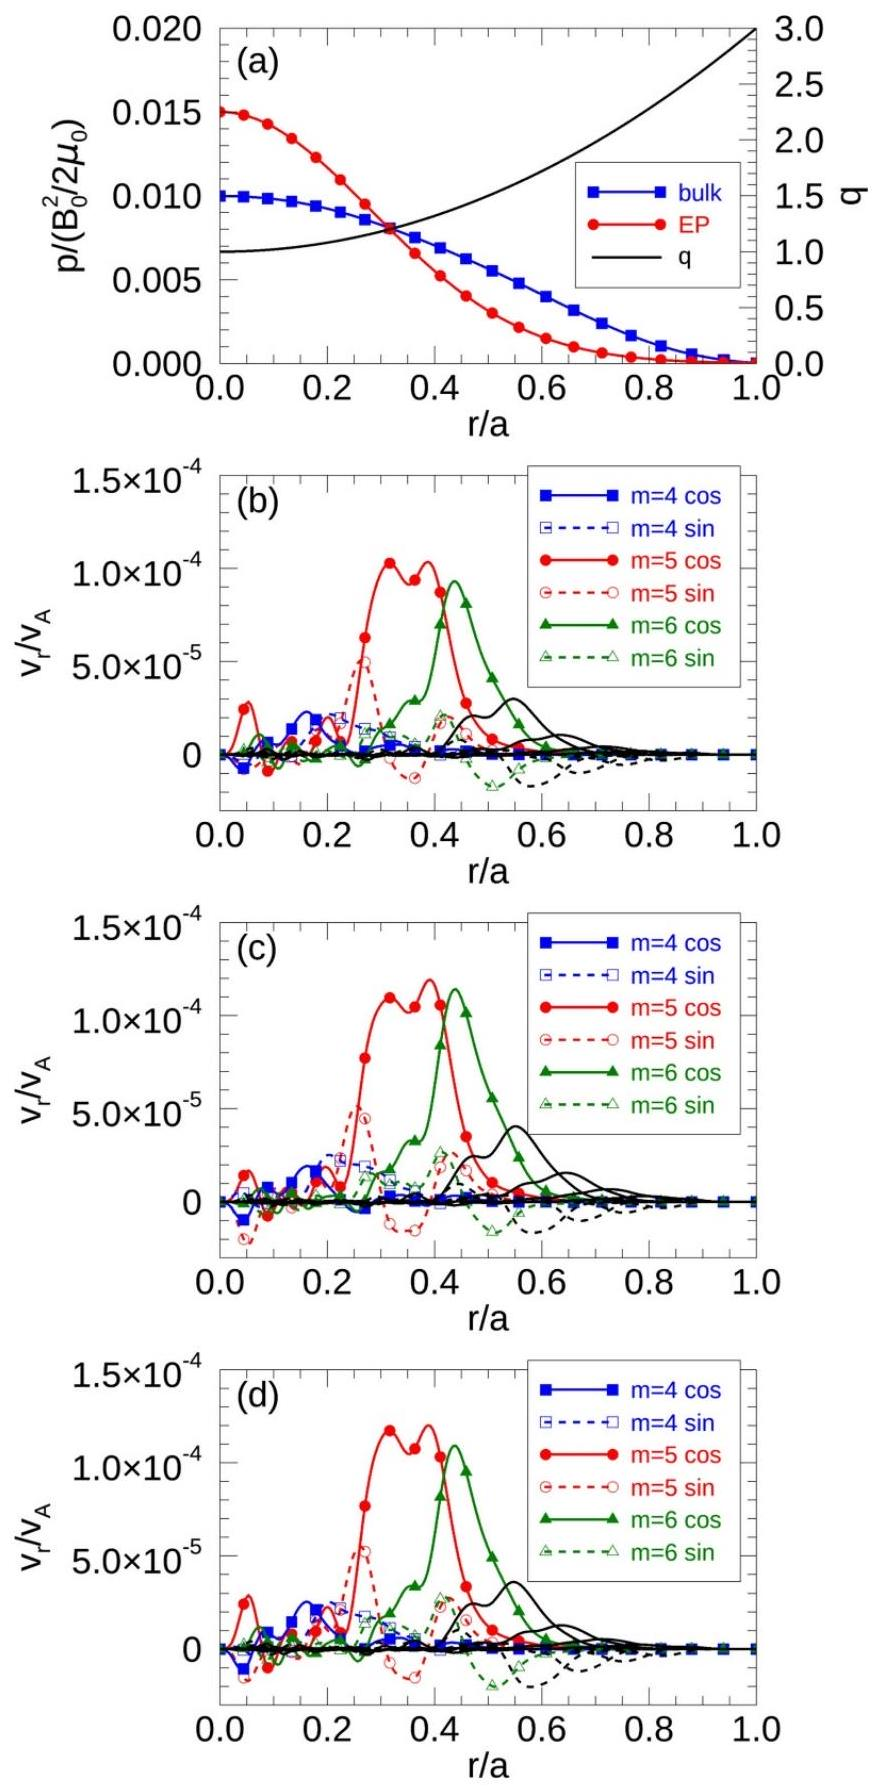
\includegraphics[max width=\textwidth, center]{2023_06_04_de2f4b8aa3fd859f006dg-05}

Figure 1. (a) Spatial profiles of bulk plasma beta, energetic ion beta (EP), and safety factor $(q)$. Spatial profiles of each poloidal harmonic of the toroidal Alfvén eigenmode (TAE) with toroidal mode number $n=4$ for radial MHD velocity simulated with (b) the conventional hybrid model, (c) the extended hybrid model with kinetic thermal ions, and (d) the extended hybrid model with kinetic thermal ions and electron temperature profile evolution. Solid (dashed) lines show $\cos (m \theta+n \varphi)[\sin (m \theta+n \varphi)]$ harmonics.

ion response for the central bulk plasma beta $1 \%$. This results in the similar growth rate between the conventional hybrid model and the extended hybrid model with kinetic thermal ions.

For the validation of the time-independent electron temperature model, we conducted another simulation where electron temperature profile evolves by the following pressure evolution equation,

$$
\begin{gathered}
\frac{\partial p_{e}}{\partial t}=-\nabla \cdot\left(p_{e} \mathbf{v}_{f e}\right)-(\gamma-1) p_{e} \nabla \cdot \mathbf{v}_{f e} \\
\mathbf{v}_{f e}=\mathbf{v}_{E \perp}+\frac{\rho_{i} v_{i \|}+\rho_{h} v_{h \|}}{\rho} \mathbf{b} .
\end{gathered}
$$

Thermal ions and energetic ions are simulated with the gyrokinetic PIC. This model is similar to that used in $[44,45]$. The spatial profile of the TAE simulated with this model is shown in figure $1(\mathrm{~d})$. We see a very similar spatial profile to those shown in figures 1(b) and (c). The real frequency and the growth rate are $\omega=0.338 \omega_{A}$ and $\gamma=0.036 \omega_{A}$ which are the same as those of the conventional hybrid model and close to those of the extended hybrid model with the time-independent electron temperature profile. This result validates the timeindependent electron temperature model used in this work for the studies of AEs.

\subsection{TAE for bulk plasma beta $1 \%$}
We compare the evolution of the TAE for different bulk plasma beta values $\beta_{\text {bulk } 0}=1 \%$ and $4 \%$ using the extended simulation model with kinetic thermal ions. Since we assumed the same density profile, the difference in bulk plasma beta arises from the different bulk plasma temperature. We show the time evolution of radial MHD velocity and energy in figure 2 for $\beta_{\mathrm{bulk} 0}=1 \%$. Figure 2 (a) shows the radial $\mathrm{MHD}$ velocity evolution for the cosine part of the $m / n=5 / 4$ harmonic which is the dominant component of the TAE as we see in figure 1(c). We see that the saturation level is $v_{r} / v_{A} \sim$ $3 \times 10^{-3}$. Figure 2 (b) shows the time evolution of energetic ion energy (EP), thermal ion energy (ion), electron energy (electron), MHD kinetic energy (kinetic), magnetic energy (magnetic), and dissipated energy (dissipation). The decrease in energetic ion energy indicates that the instability is driven by energetic ions. Figure 2(c) compares the evolution of absolute value for energetic ion energy, thermal ion energy, electron energy, and MHD kinetic energy in logarithmic scale. We see that all the energy components grow with the same growth rate. Since the sign of thermal ion and electron energy is positive in figure 2(b), both thermal ions and electrons absorb energy from the TAE. The absolute values of energy variation are comparable between thermal ions and electrons. This suggests that the interaction between thermal ions and the TAE is fluid-like and the resonance plays only a minor role. This will be confirmed with the distribution function analyses described below.

We have analyzed the variations of energetic ion distribution function $(\delta f)$ in phase space $\left(P_{\varphi}, E, \mu\right)$ where $P_{\varphi}$, $E$, and $\mu$ represent toroidal canonical momentum, kinetic energy, and magnetic moment, respectively, with the definition $P_{\varphi}=e_{h} \Psi+m_{h} R v_{\|} b_{\varphi}, E=\frac{1}{2} m_{h} v^{2}$, and $\mu=\frac{1}{2} m_{h} v_{\perp}^{2} / B$. Magnetic moment $\mu$ is an adiabatic invariant for the interaction with AEs whose frequency is sufficiently lower than the ion Larmor frequency. The poloidal magnetic flux $\Psi$ is chosen
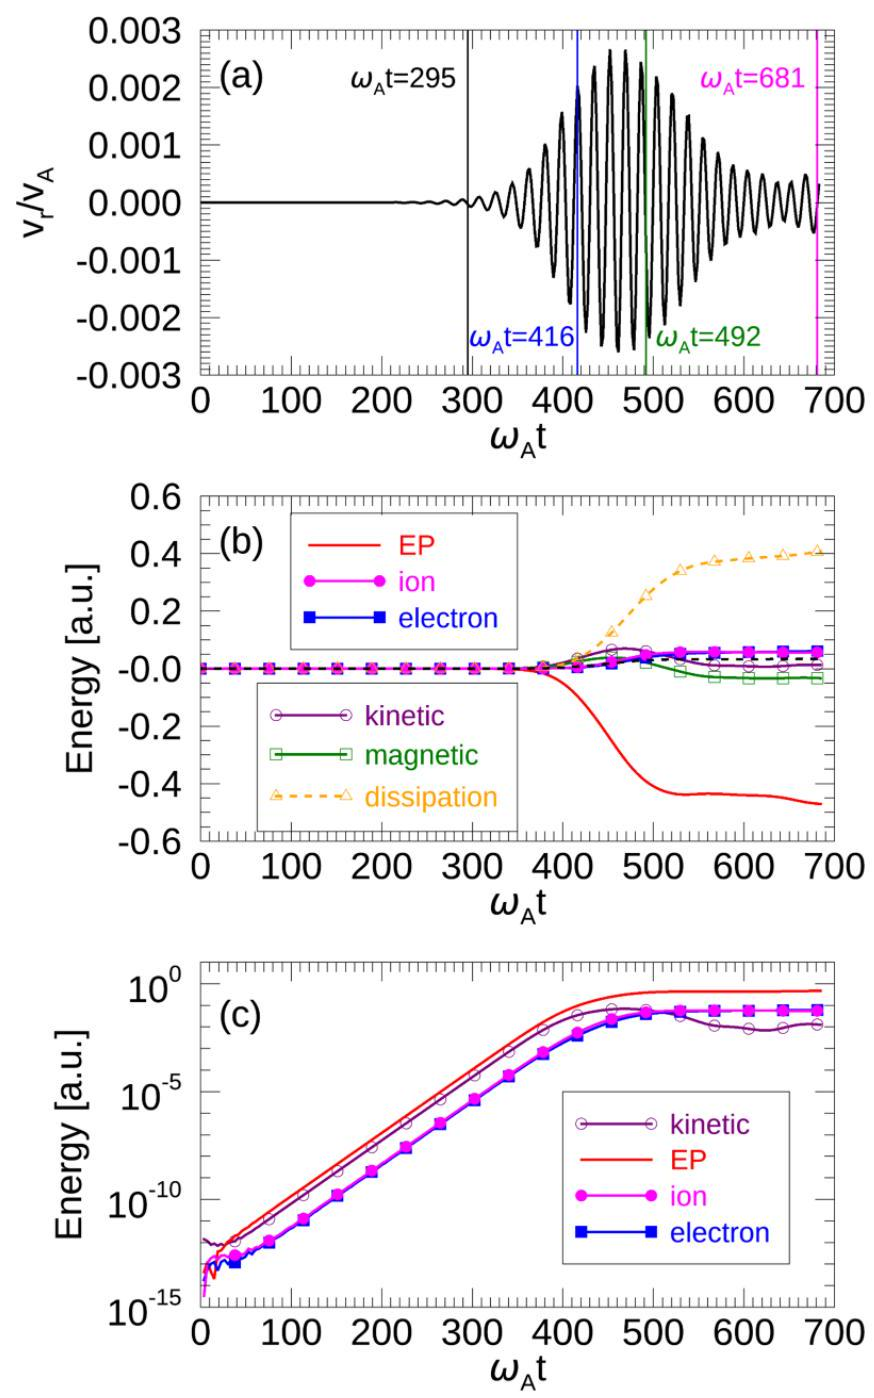
\includegraphics[max width=\textwidth, center]{2023_06_04_de2f4b8aa3fd859f006dg-06}

Figure 2. (a) Radial MHD velocity evolution for the cosine part of the $m / n=5 / 4$ harmonic shown in figure 1(c) for $\beta_{\text {bulk } 0}=1 \%$. (b) Time evolution of variations for energetic ion energy (EP), thermal ion energy (ion), electron energy (electron), MHD kinetic energy (kinetic), magnetic energy (magnetic), and dissipated energy (dissipation) for $\beta_{\text {bulk } 0}=1 \%$. Panel (c) compares the evolution of absolute value for energetic ion energy, thermal ion energy, electron energy, and MHD kinetic energy in logarithmic scale.

to be $\Psi=\Psi_{0}$ at the plasma center and $\Psi=0$ at the plasma edge. The subscript ' $h$ ' denotes energetic ion, and $b_{\varphi}$ is the $\varphi$ component of the magnetic field unit vector.

The variations of energetic ion distribution function $(\delta f)$ in $\left(P_{\varphi}, E\right)$ space with $\mu=0$ are shown in figure 3 for $\omega_{A} t=681$ in the run for $\beta_{\text {bulk } 0}=1 \%$. We chose $\mu=0$ because the absolute value of $\delta f$ is large. The blue and red regions shown in figures 3(a) and (b) represent $\delta f<0$ and $\delta f>0$, respectively. The resonance condition is given by (e.g. [53]):

$$
\omega-n \omega_{\varphi}-L \omega_{\vartheta}=0
$$

where $\omega_{\varphi}$ and $\omega_{\vartheta}$ are particle orbit frequencies in toroidal and poloidal directions, respectively, and the poloidal resonance number $L$ is an integer. We measured the particle orbit
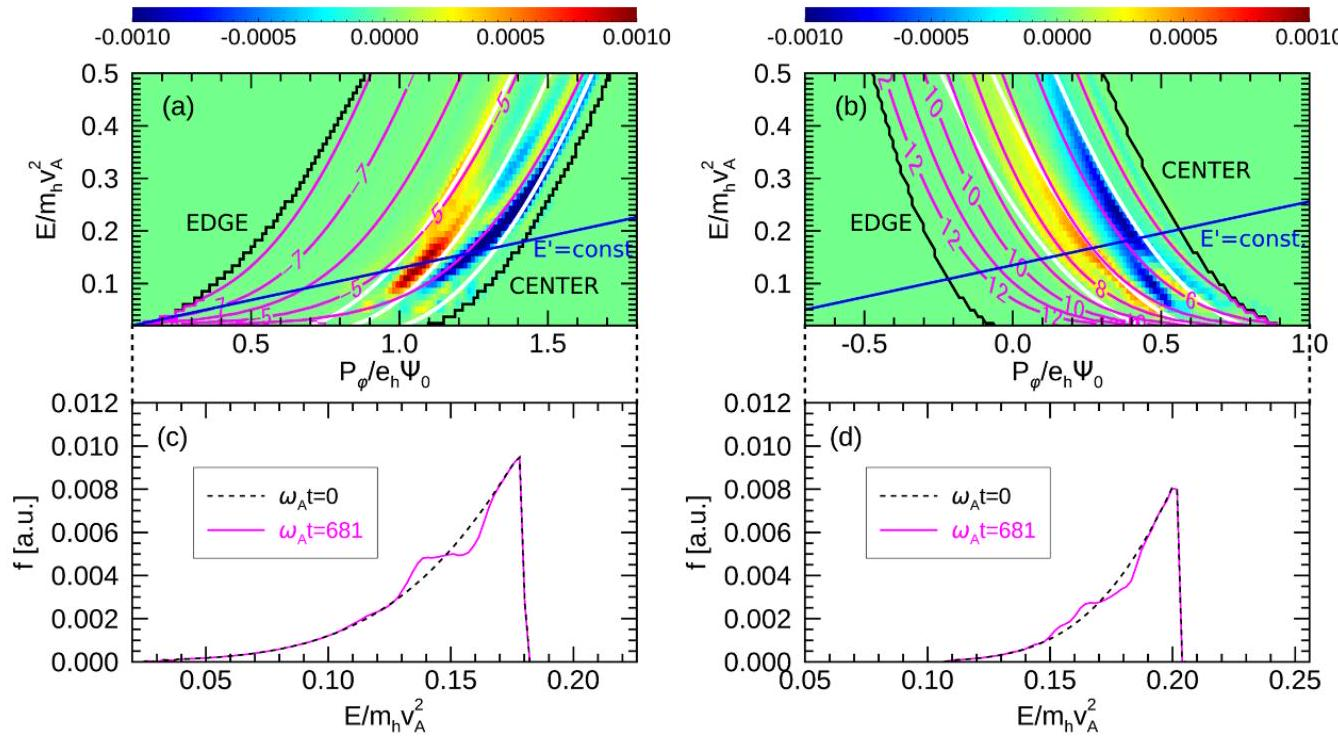
\includegraphics[max width=\textwidth, center]{2023_06_04_de2f4b8aa3fd859f006dg-07}

Figure 3. Variations of energetic ion distribution function in $\left(P_{\varphi}, E\right)$ space with $\mu=0$ are shown in color for (a) co-going particles to the plasma current and (b) counter-going particles at $\omega_{A} t=681$ in the run for $\beta_{\text {bulk } 0}=1 \%$. Magenta lines represent resonance with the TAE with poloidal resonance number $L$ labeled in the figure. White lines represent the TAE gap locations for toroidal mode number $n=4$ with $q=9 / 8,11 / 8$, and $13 / 8$. Blue lines represent $E^{\prime}=$ const. which is conserved during the wave-particle interaction neglecting the time variation of the mode amplitude and frequency. Energetic ion distribution functions along the $E^{\prime}=$ const. lines shown in panels (a) and (b) are compared between $\omega_{A} t=0$ and 681 for (c) co-going particles and (d) counter-going particles. Dashed lines connecting panel (a, b) to (c, d), respectively, indicate the range of $P_{\varphi}$ which corresponds to the horizontal axis $(E)$ of panels (c, d).
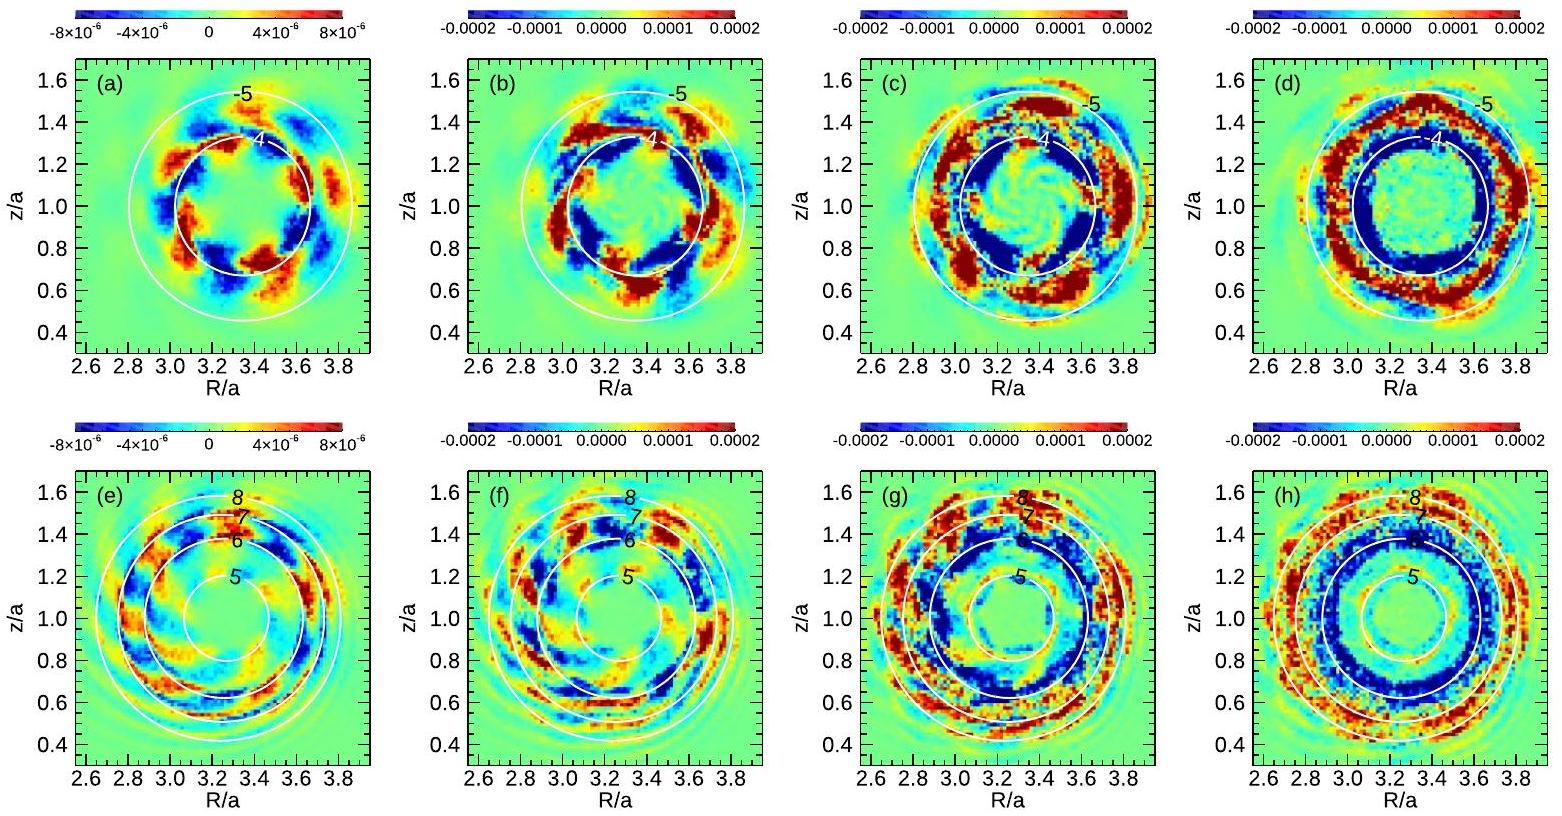
\includegraphics[max width=\textwidth, center]{2023_06_04_de2f4b8aa3fd859f006dg-07(1)}

Figure 4. Energetic ion distribution function fluctuations in a poloidal plane $\left(R_{0}-0.65 a \leqslant R \leqslant R_{0}+0.75 a, z_{0}-0.7 a \leqslant z \leqslant z_{0}\right.$ $+0.7 a, \varphi=0$ ) with $R_{0}=3.2 a$ and $z_{0}=a$ for (a), (e) $\omega_{A} t=295$, (b), (f) $\omega_{A} t=416$, (c, g) $\omega_{A} t=492$, (d, h) $\omega_{A} t=681$ in the run for $\beta_{\text {bulk } 0}=1 \%$. Particle kinetic energy is chosen for the constant $E^{\prime}$ which are shown in figure 3 and magnetic moment $\mu=0$. The top (bottom) panels show co-going (counter-going) particles to the plasma current. Resonant particle orbits are projected on the poloidal plane with the poloidal resonance number $L$ labeled in the figure.

frequencies and defined the following function of $\omega_{\varphi}$ and $\omega_{\vartheta}:$

$$
F\left(\omega_{\varphi}, \omega_{\vartheta}\right)=\left(\omega-n \omega_{\varphi}\right) / \omega_{\vartheta}
$$

in $\left(P_{\varphi}, E, \mu\right)$ space. The resonance condition is $F\left(\omega_{\varphi}, \omega_{\vartheta}\right)=L$. Magenta lines shown in figures 3(a) and (b) are contours of $F\left(\omega_{\varphi}, \omega_{\vartheta}\right)$ with levels $L$ labeled in the figure, which represent the resonance with the TAE. White lines represent the TAE gap locations for toroidal mode number $n=4$ with $q=9 / 8,11 / 8$,
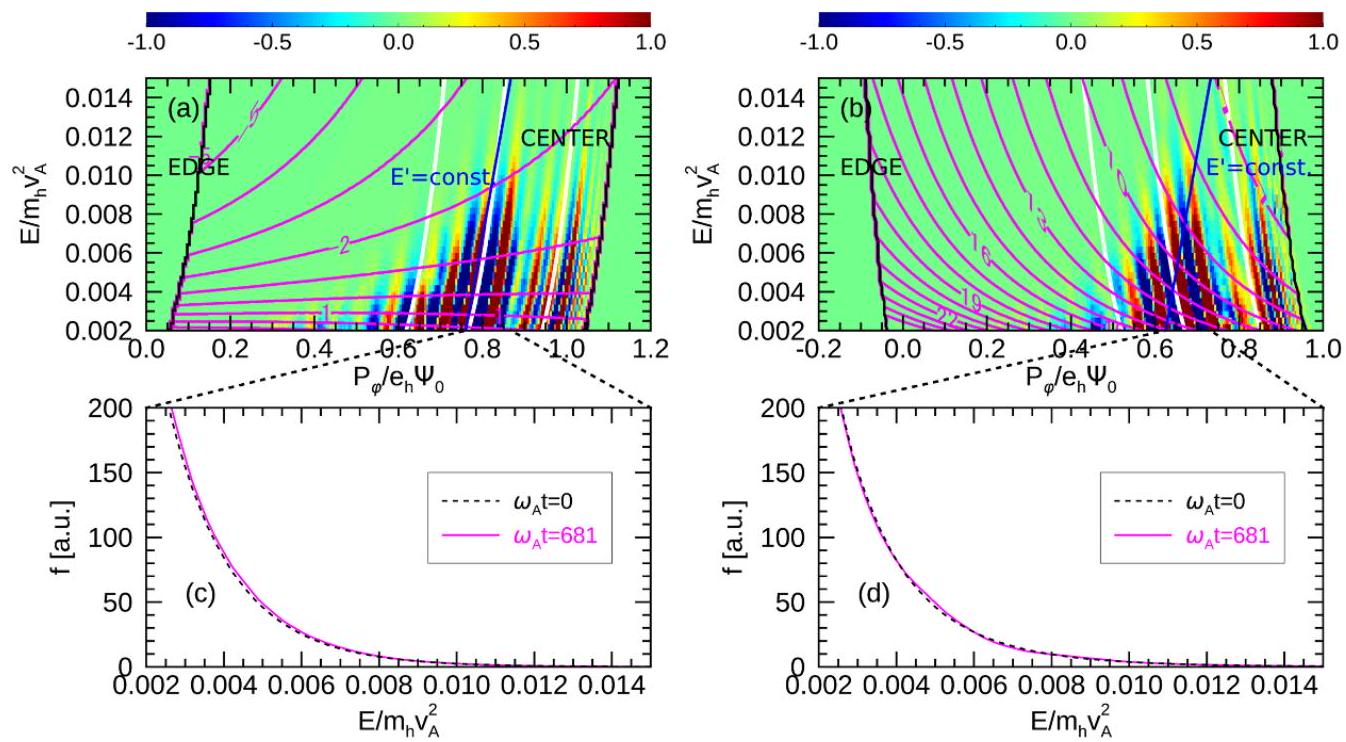
\includegraphics[max width=\textwidth, center]{2023_06_04_de2f4b8aa3fd859f006dg-08}

Figure 5. Variations of thermal ion distribution function in $\left(P_{\varphi}, E\right)$ space with $\mu=0$ are shown in color for (a) co-going particles to the plasma current and (b) counter-going particles at $\omega_{A} t=681$ in the run for $\beta_{\text {bulk } 0}=1 \%$. Magenta lines represent resonance with the TAE with poloidal resonance number $L$ labeled in the figure. White lines represent the TAE gap locations for toroidal mode number $n=4$ with $q=9 / 8,11 / 8$, and $13 / 8$. Blue lines represent $E^{\prime}=$ const. which is conserved during the wave-particle interaction neglecting the time variation of the mode amplitude and frequency. Thermal ion distribution functions along the $E^{\prime}=$ const. lines shown in panels (a) and (b) are compared between $\omega_{A} t=0$ and 681 for (c) co-going particles and (d) counter-going particles. Dashed lines connecting panel (a, b) to (c, d), respectively, indicate the range of $P_{\varphi}$ which corresponds to the horizontal axis $(E)$ of panels $(\mathrm{c}, \mathrm{d})$.
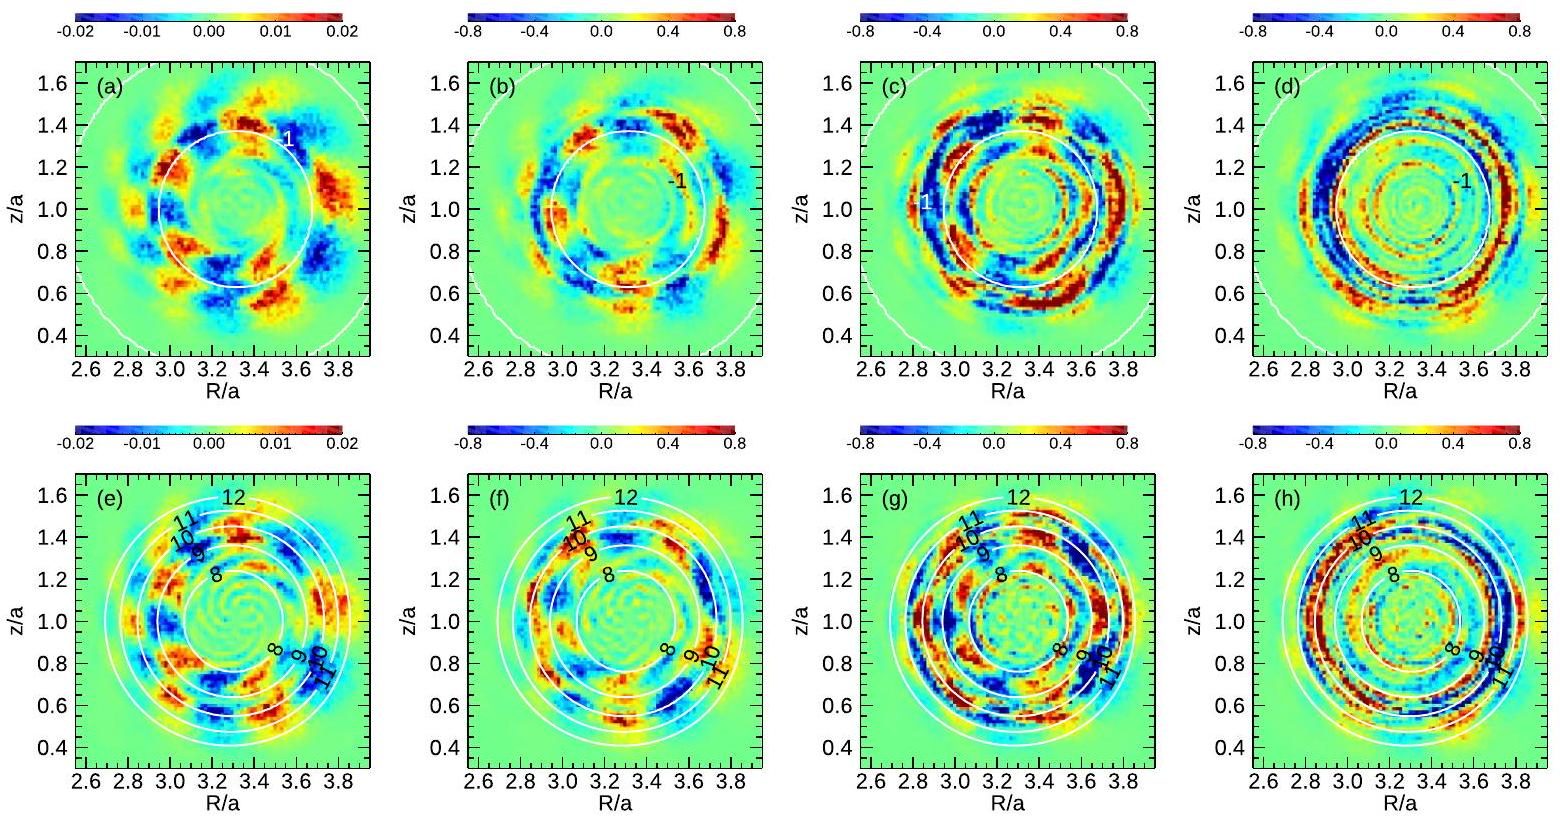
\includegraphics[max width=\textwidth, center]{2023_06_04_de2f4b8aa3fd859f006dg-08(1)}

Figure 6. Thermal ion distribution function fluctuations in a poloidal plane $\left(R_{0}-0.65 a \leqslant R \leqslant R_{0}+0.75 a, z_{0}-0.7 a \leqslant z \leqslant z_{0}\right.$ $+0.7 a, \varphi=0)$ with $R_{0}=3.2 a$ and $z_{0}=a$ for (a, e) $\omega_{A} t=295$, (b) (f) $\omega_{A} t=416$, (c, g) $\omega_{A} t=492$, (d, h) $\omega_{A} t=681$ in the run for $\beta_{\text {bulk } 0}=1 \%$. Particle kinetic energy is $E=5.9 \times 10^{-3} m_{h} v_{A}^{2}$ and magnetic moment $\mu=0$. The top (bottom) panels show co-going (counter-going) particles to the plasma current. Resonant particle orbits are projected on the poloidal plane with the poloidal resonance number $L$ labeled in the figure.

and $13 / 8$ whose radii are $r / a=0.25,0.43$, and 0.56 , respectively. We see in figure $1(\mathrm{c})$ that the TAE has a substantial amplitude in the region with $9 / 8 \leqslant q \leqslant 13 / 8$. We see in the figure that the large $|\delta f|$ appear along the resonance lines (magenta) and close to the TAE location represented by the gap lines (white). During the wave-particle interaction, $E^{\prime}=E-\frac{\omega}{n} P_{\varphi}$ is conserved neglecting the time variation of the mode amplitude and frequency [53, 54]. Blue lines shown in figures 3(a) and (b) represent $E^{\prime}=$ const. Energetic ion distribution functions along the $E^{\prime}=$ const. lines shown in figures 3(a) and (b) are compared between $\omega_{A} t=0$ and 681 for (c) co-going particles and (d) counter-going particles. We should notice that the distribution function gradient with respect to kinetic energy $E$ $(=d f / d E)$ along the $E^{\prime}=$ const. line represents the free energy source for the inverse Landau damping because the following relationship holds [53]:

$$
\left.\frac{\partial f}{\partial E}\right|_{E^{\prime}}=\frac{\partial f}{\partial E}+\frac{d P_{\varphi}}{d E} \frac{\partial f}{\partial P_{\varphi}}=\frac{\partial f}{\partial E}+\frac{n}{\omega} \frac{\partial f}{\partial P_{\varphi}} .
$$

We see in figures 3(c) and (d) that the distribution function has positive gradient $(d f / d E>0)$ along the $E^{\prime}=$ const. lines at $\omega_{A} t=0$. This causes the inverse Landau damping and the growth of the TAE. We see the flattening of the energetic ion distribution function due to the interaction with the TAE at $\omega_{A} t=681$. The flattening of the distribution function can be attributed to the particle trapping by the TAE.

We show in figure 4 the energetic ion distribution function fluctuations in a poloidal plane $\left(R_{0}-0.65 a \leqslant R \leqslant R_{0}+\right.$ $\left.0.75 a, z_{0}-0.7 a \leqslant z \leqslant z_{0}+0.7 a, \varphi=0\right)$ with $R_{0}=3.2 a$ and $z_{0}=a$ for different times. Particle kinetic energy is chosen for the constant $E^{\prime}$ values for co- and counter-going particles which are shown in figure 3 and magnetic moment $\mu=0$. Resonant particle orbits are projected on the poloidal plane with the poloidal resonance number $L$ labeled in the figure. For the linearly growing phase of the TAE shown in figures 4(a) and (e), we see that the distribution function fluctuations have the same poloidal mode numbers as the poloidal resonance numbers labeled in the figures. This indicates that the resonance is taking place. Just after the saturation of the instability shown in figures 4(c) and (g), we see the blue regions inside the resonant orbits and the red regions outside the resonant orbits. Blue and red regions represent $\delta f<0$ and $\delta f>0$, respectively. This indicates the flattening of the distribution function at the resonances caused by particle trapping. Figures 4(b) and (f) show $\delta f$ at the beginning of the nonlinear saturation phase where particle trapping is starting. As the TAE amplitude decreases after the distribution flattening, the distribution function is kept flattened and becomes uniform in the poloidal direction as shown in figures $4(\mathrm{~d})$ and (h).

The variations of thermal ion distribution function $(\delta f)$ are shown in figure 5 in $\left(P_{\varphi}, E\right)$ space with $\mu=0$ at $\omega_{A} t=681$ in the run for $\beta_{\text {bulk } 0}=1 \%$. The blue and red regions shown in figures 5(a) and (b) represent $\delta f<0$ and $\delta f>0$, respectively. Magenta lines represent resonance with the TAE with poloidal resonance number $L$ labeled in the figure. White lines represent the TAE gap locations for toroidal mode number $n=4$ with $q=9 / 8,11 / 8$, and $13 / 8$. We see in the figure that the large absolute value of $\delta f$ appear close to the TAE location represented by the gap lines (white). The large $|\delta f|$ regions do not follow the resonance curves shown in magenta. This indicates that the resonance does not play a dominant role in the interaction between the TAE and thermal ions. Thermal ion distribution functions along the $E^{\prime}=$ const. lines shown in figures 5 (a) and (b) are compared between $\omega_{A} t=0$ and 681 for (c) co-going particles and (d) counter-going particles. The variations of thermal ion distribution functions are small indicating a weak interaction between the TAE and thermal ions.
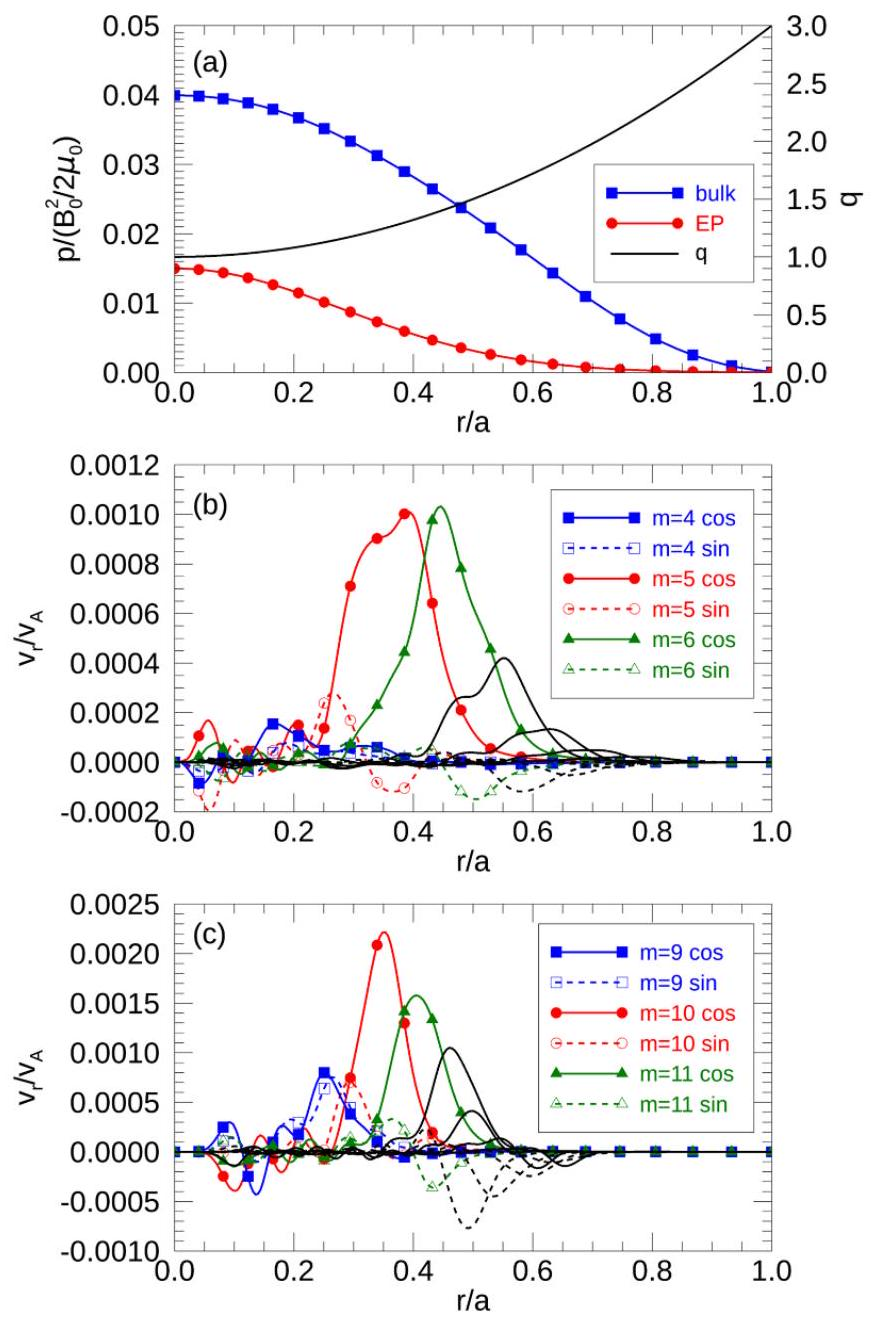
\includegraphics[max width=\textwidth, center]{2023_06_04_de2f4b8aa3fd859f006dg-09}

Figure 7. (a) Spatial profiles of bulk plasma beta, energetic ion beta (EP), and safety factor $(q)$. Spatial profiles of each poloidal harmonic of the TAEs with toroidal mode number (b) $n=4$ and (c) $n=8$ for radial MHD velocity. Solid (dashed) lines show $\cos (m \theta+n \varphi)[\sin (m \theta+n \varphi)]$ harmonics.

We show in figure 6 the thermal ion distribution function fluctuations in the $(R, z)$ plane for different times. Particle kinetic energy is chosen for the constant $E=5.9 \times 10^{-3} m_{h} v_{A}^{2}$. We do not collect particles with $E^{\prime}=$ const. for this analysis because we cannot cover the $(R, z)$ plane with the $E^{\prime}=$ const. condition which has a steep gradient in $P_{\varphi}$ as shown in figures 5(a) and (b). Resonant particle orbits are projected on the $(R, z)$ plane with the poloidal resonance number $L$ labeled in the figure. For the linearly growing phase of the TAE shown in figures 6(a) and (e), we see that the distribution function fluctuations do not have the same poloidal mode numbers as the poloidal resonance numbers. This indicates that the resonance is not a dominant factor for the distribution function fluctuations. This property does not change for the different times shown in the other panels of figure 6 . The thermal ion distribution function fluctuations for the linearly growing phase of the TAE shown in figures 6(a) and (e) have the same poloidal mode numbers $(m=4-6)$ as the TAE spatial profile. This indicates the fluid-like interaction of thermal ions with the TAE. It is also
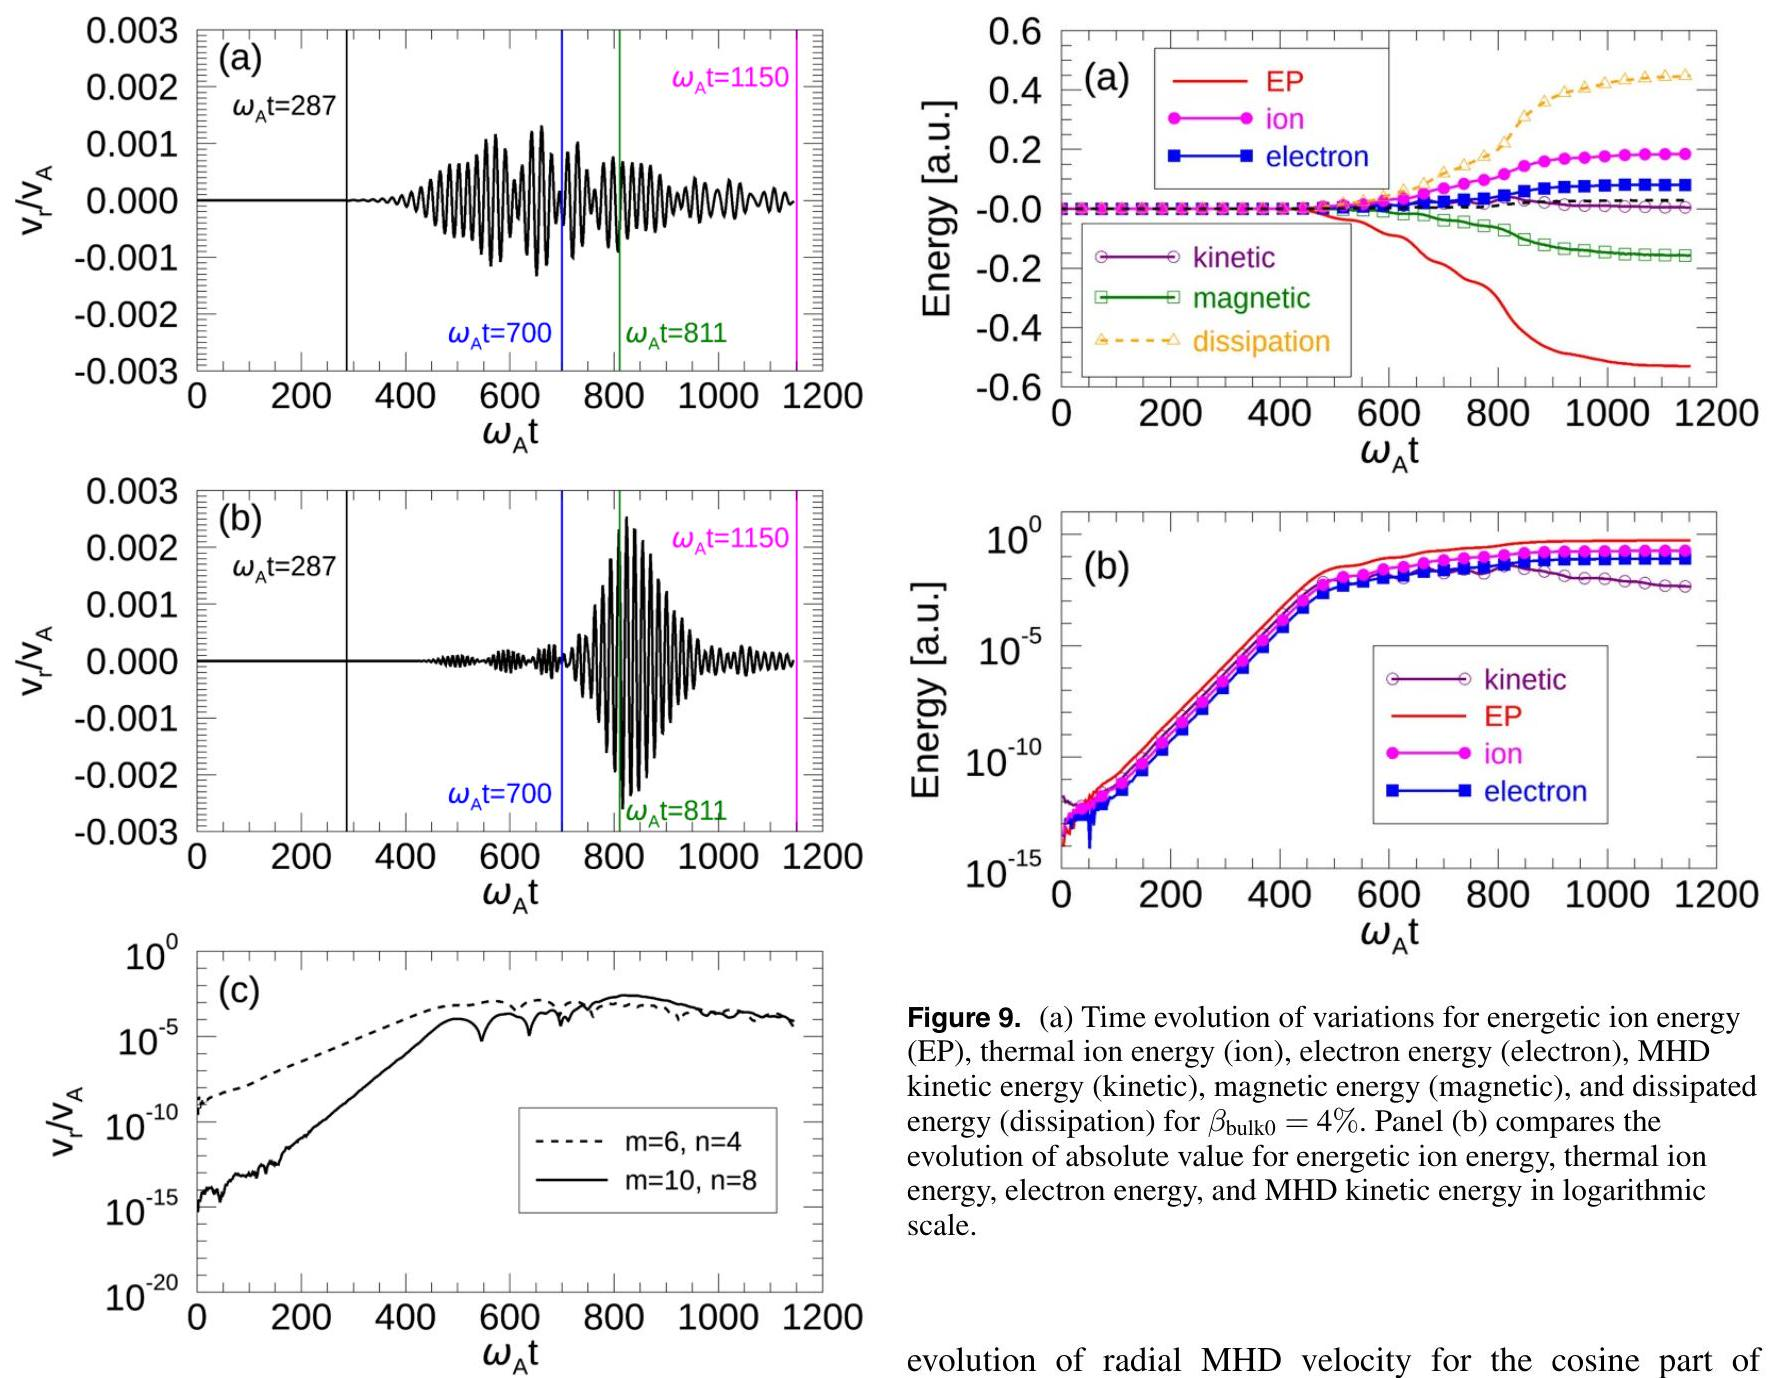
\includegraphics[max width=\textwidth, center]{2023_06_04_de2f4b8aa3fd859f006dg-10}

Figure 9. (a) Time evolution of variations for energetic ion energy (EP), thermal ion energy (ion), electron energy (electron), MHD kinetic energy (kinetic), magnetic energy (magnetic), and dissipated energy (dissipation) for $\beta_{\text {bulk } 0}=4 \%$. Panel (b) compares the evolution of absolute value for energetic ion energy, thermal ion energy, electron energy, and MHD kinetic energy in logarithmic scale.

evolution of radial MHD velocity for the cosine part of $m / n=6 / 4$ harmonic and $m / n=10 / 8$ harmonic, respectively.

Figure 8. Radial MHD velocity evolution for the cosine part of (a) $m / n=6 / 4$ and (b) $m / n=10 / 8$ harmonics shown in figures 7(b) and (c), respectively, for $\beta_{\text {bulk } 0}=4 \%$. Panel (c) compares the evolution of absolute value for the radial MHD velocity harmonics in logarithmic scale.

interesting that small scale variations in the radial direction are formed in the nonlinear phase, which are seen in figures 5(a) and (b), and figures 6(d) and (h).

\subsection{TAEs for bulk plasma beta $4 \%$}
In this subsection, we investigate another case with bulk plasma beta $\beta_{\text {bulk } 0}=4 \%$ using the extended simulation model with kinetic thermal ions. We show the spatial profiles of the bulk plasma beta, energetic ion beta, and safety factor in figure 7 (a). The bulk plasma density is uniform. Since we assumed the same density profile as the run for $\beta_{\text {bulk } 0}=1 \%$ presented in the previous subsection, the higher bulk plasma beta arises from the higher bulk plasma temperature. The radial MHD velocity profiles are shown in figures 7 (b) and (c) for $n=4$ and $n=8$ TAEs which appear in the simulation.

We show the time evolution of radial MHD velocity in figure 8 for $\beta_{\text {bulk } 0}=4 \%$. Figures 8 (a) and (b) show the time

The most unstable mode in the linearly growing phase is the $n=4$ TAE. The saturation amplitude of $m / n=6 / 4$ harmonic is $v_{r} / v_{A} \sim 1 \times 10^{-3}$ which is lower than that for $\beta_{\text {bulk } 0}=1 \%$. Figure 8(c) compares the evolution of the $m / n=6 / 4$ and $10 / 8$ harmonics in logarithmic scale. The growth rate of the $m / n=10 / 8$ harmonic in the linearly growing phase is twice that of the $m / n=6 / 4$ harmonic. This indicates that the $n=8$ mode is generated from the $n=4$ mode through the MHD nonlinearity. After the saturation of the $n=4 \mathrm{TAE}$, the $n=8 \mathrm{TAE}$ becomes unstable and grows to a larger amplitude than the $n=4$ TAE. The $n=8$ TAE may be destabilized by the energetic ion redistribution brought about by the $n=4$ TAE.

Figure 9(a) shows the time evolution of variations for energetic ion energy (EP), thermal ion energy (ion), electron energy (electron), MHD kinetic energy (kinetic), magnetic energy (magnetic), and dissipated energy (dissipation). The decrease in energetic ion energy indicates that the instability is driven by energetic ions. Figure 9(b) compares the absolute value of variations for energetic ion energy, thermal ion energy, electron energy, and MHD kinetic energy in logarithmic scale. We see that all the energy components grow with the same growth rate. The positive sign of thermal ion and electron energy which we see in figure 9 (a) indicates that both thermal ions and electrons absorb energy from the TAEs. The
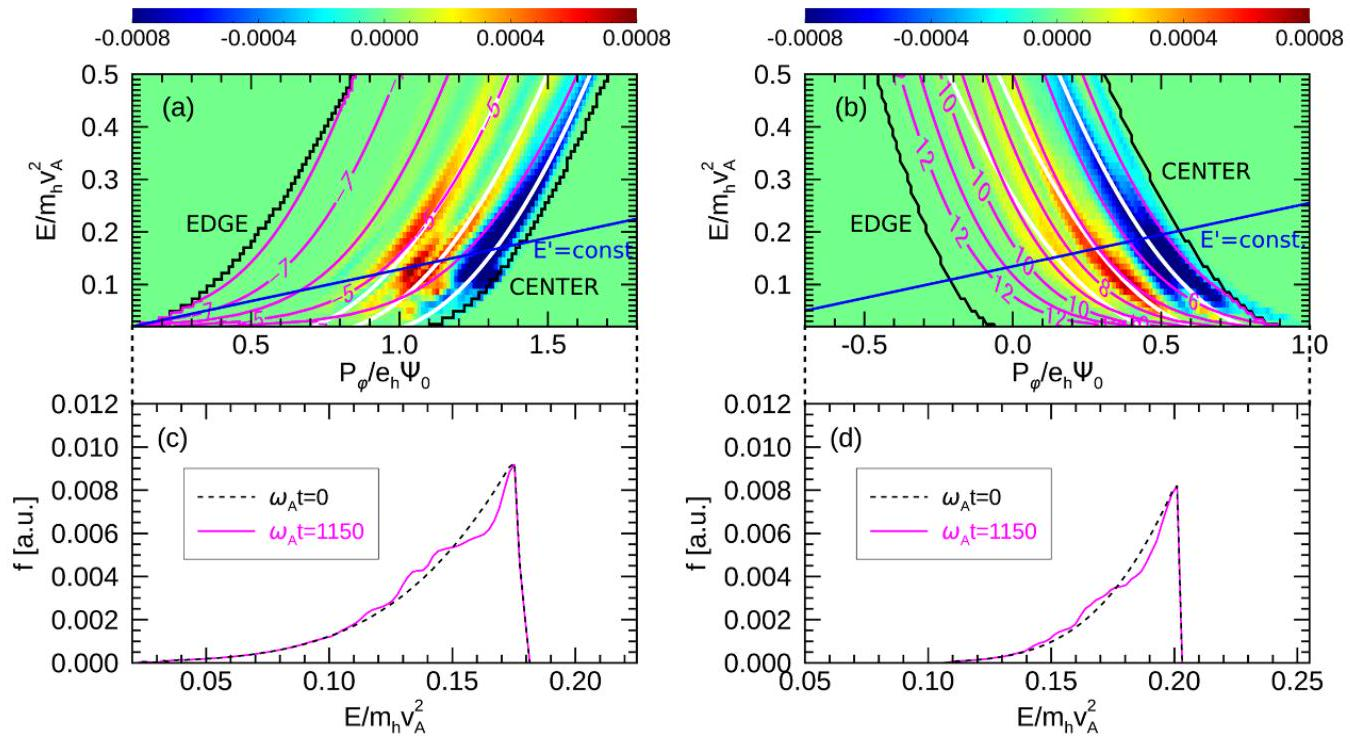
\includegraphics[max width=\textwidth, center]{2023_06_04_de2f4b8aa3fd859f006dg-11}

Figure 10. Variations of energetic ion distribution function in $\left(P_{\varphi}, E\right)$ space with $\mu=0$ are shown in color for (a) co-going particles to the plasma current and (b) counter-going particles at $\omega_{A} t=1150$ in the run for $\beta_{\text {bulk } 0}=4 \%$. Magenta lines represent resonance with the $n=4$ TAE with poloidal resonance number $L$ labeled in the figure. White lines represent the TAE gap locations for toroidal mode number $n=4$ with $q=9 / 8,11 / 8$, and $13 / 8$. Blue lines represent $E^{\prime}=$ const. which is conserved during the wave-particle interaction with the $n=4$ TAE neglecting the time variation of the mode amplitude and frequency. Energetic ion distribution functions along the $E^{\prime}=$ const. lines shown in panels (a, b) are compared between $\omega_{A} t=0$ and 1150 for (c) co-going particles and (d) counter-going particles. Dashed lines connecting panel $(\mathrm{a}, \mathrm{b})$ to $(\mathrm{c}, \mathrm{d})$, respectively, indicate the range of $P_{\varphi}$ which corresponds to the horizontal axis $(E)$ of panels (c) and (d).
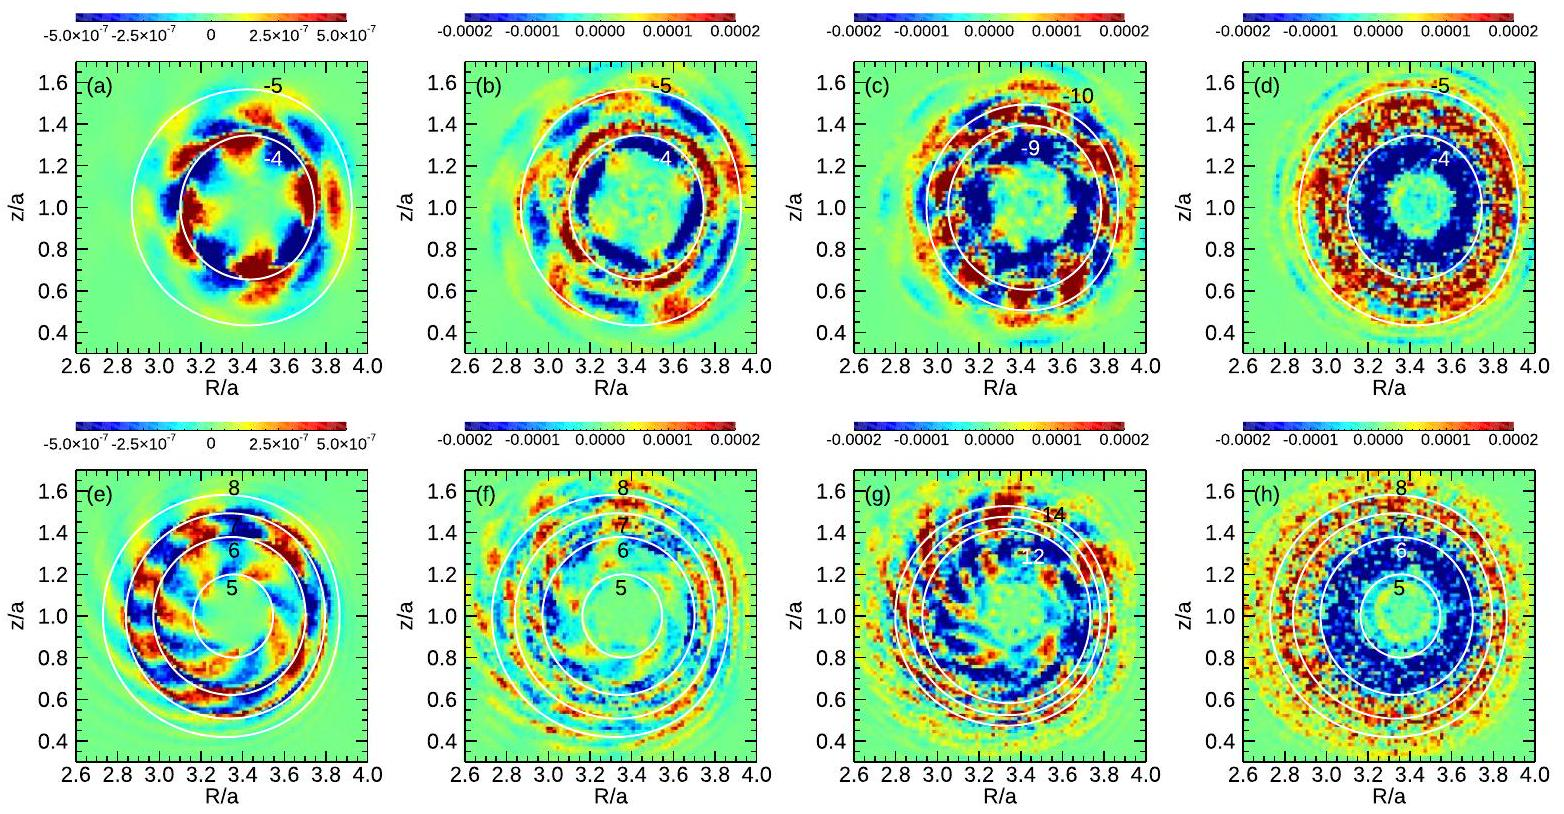
\includegraphics[max width=\textwidth, center]{2023_06_04_de2f4b8aa3fd859f006dg-11(1)}

Figure 11. Energetic ion distribution function fluctuations in a poloidal plane $\left(R_{0}-0.65 a \leqslant R \leqslant R_{0}+0.75 a, z_{0}-0.7 a \leqslant z \leqslant z_{0}\right.$ $+0.7 a, \varphi=0)$ with $R_{0}=3.2 a$ and $z_{0}=a$ for $(\mathrm{a}, \mathrm{e}) \omega_{A} t=287,(\mathrm{~b}, \mathrm{f}) \omega_{A} t=700,(\mathrm{c}, \mathrm{g}) \omega_{A} t=811,(\mathrm{~d}, \mathrm{~h}) \omega_{A} t=1150$ in the run for $\beta_{\text {bulk } 0}=4 \%$. Particle kinetic energy is chosen for the constant $E^{\prime}$ which are shown in figure 10 and magnetic moment $\mu=0$. The top (bottom) panels show co-going (counter-going) particles to the plasma current. Resonant particle orbits are projected on the poloidal plane with the poloidal resonance number $L$ labeled in $(\mathrm{c})$ and $(\mathrm{g})$ for the $n=8$ TAE and in the other panels for the $n=4$ TAE.

absolute value of energy variation for thermal ions is larger than that for electrons. In the run for $\beta_{\mathrm{bulk} 0}=1 \%$, the energy variations are comparable between thermal ions and electrons as shown in figure 2 . The larger increase in thermal ion energy for $\beta_{\text {bulk } 0}=4 \%$ can be attributed to stronger Landau damping of thermal ions with higher thermal ion temperature. This will be clarified with the distribution function analyses described below.

We have analyzed the variations of energetic ion distribution function $(\delta f)$ in phase space $\left(P_{\varphi}, E, \mu\right)$. The variations of energetic ion distribution function in $\left(P_{\varphi}, E\right)$ space with $\mu=0$ are shown in figure 10 for $\omega_{A} t=1150$ in
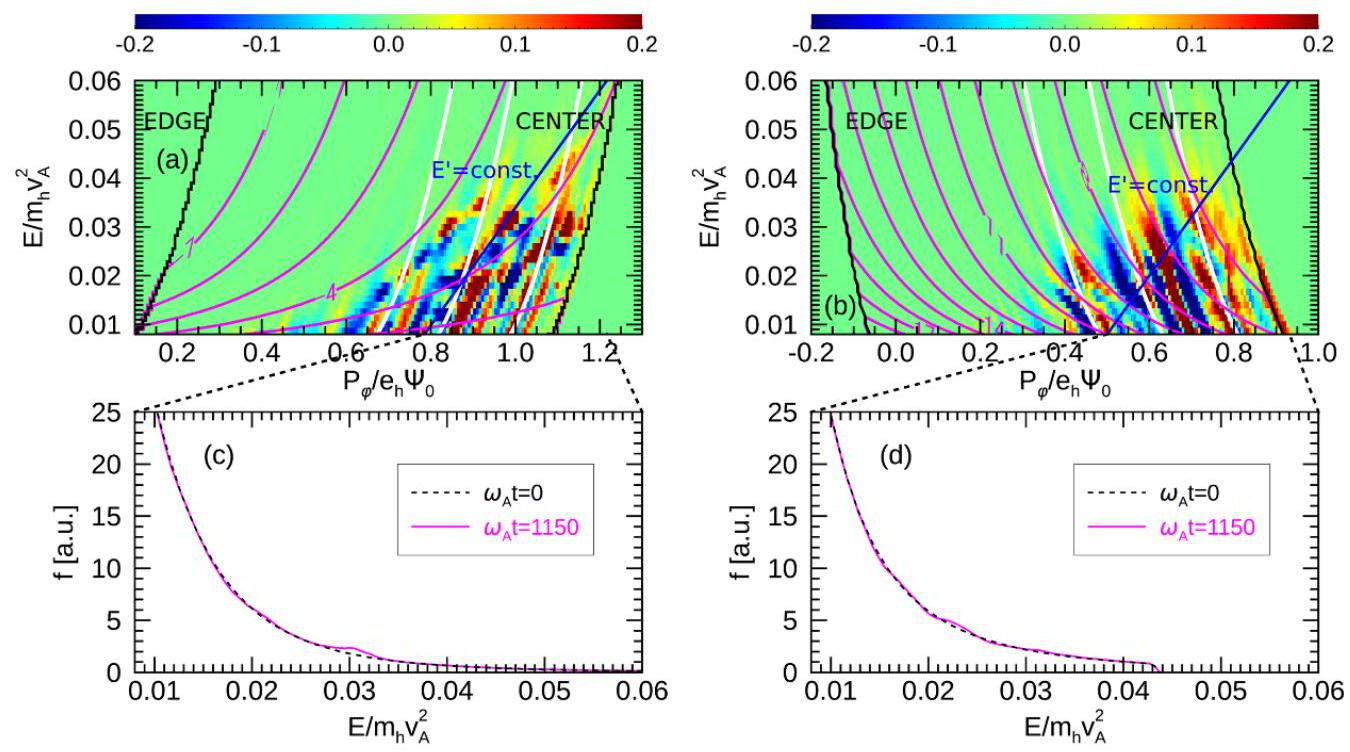
\includegraphics[max width=\textwidth, center]{2023_06_04_de2f4b8aa3fd859f006dg-12}

Figure 12. Variations of thermal ion distribution function in $\left(P_{\varphi}, E\right)$ space with $\mu=0$ are shown in color for (a) co-going particles to the plasma current and (b) counter-going particles at $\omega_{A} t=1150$ in the run for $\beta_{\text {bulk } 0}=4 \%$. Magenta lines represent resonance with the TAE with poloidal resonance number $L$ labeled in the figure. White lines represent the TAE gap locations for toroidal mode number $n=4$ with $q=9 / 8,11 / 8$, and $13 / 8$. Blue lines represent $E^{\prime}=$ const. which is conserved during the wave-particle interaction neglecting the time variation of the mode amplitude and frequency. Thermal ion distribution functions along the $E^{\prime}=$ const. lines shown in panels (a, b) are compared between $\omega_{A} t=0$ and 1150 for (c) co-going particles and (d) counter-going particles. Dashed lines connecting panel (a, b) to $(\mathrm{c}, \mathrm{d})$, respectively, indicate the range of $P_{\varphi}$ which corresponds to the horizontal axis $(E)$ of panels $(c, \mathrm{~d})$.

the run for $\beta_{\text {bulk } 0}=4 \%$. The blue and red regions shown in figures $10(\mathrm{a}, \mathrm{b})$ represent $\delta f<0$ and $\delta f>0$, respectively. Magenta lines represent resonance with the $n=4$ TAE with poloidal resonance number $L$ labeled in the figure. Blue lines represent $E^{\prime}=$ const. which is conserved during the waveparticle interaction with the $n=4$ TAE neglecting the time variation of the mode amplitude and frequency. Energetic ion distribution functions along the $E^{\prime}=$ const. lines shown in figures $10(\mathrm{a}, \mathrm{b})$ are compared between $\omega_{A} t=0$ and 1150 for (c) co-going particles and (d) counter-going particles. We see in the figure that the large-scale redistribution occurs due to the interaction with the multiple TAEs with $n=4$ and $n=8$.

We show in figure 11 the energetic ion distribution function fluctuations in the poloidal plane for different times. Particle kinetic energy is chosen for the constant $E^{\prime}$ which are shown in figure 10 and magnetic moment $\mu=0$. Resonant particle orbits are projected on the poloidal plane with the poloidal resonance number $L$ labeled in the figure. For the linearly growing phase of the TAE shown in figures 11(a) and (e), we see that the distribution function variations have the same poloidal mode numbers as the poloidal resonance numbers. This indicates that the resonance is occurring. At $\omega_{A} t=700$ shown in figures 11(b) and (f) just before the significant growth of the $n=8$ mode, blue regions with $\delta f<0$ (red regions with $\delta f>0$ ) are appearing inside (outside) of each resonance. This indicates the particle trapping by the $n=4$ TAE. However, at $\omega_{A} t=811$ shown in figures $11(\mathrm{c}, \mathrm{g})$, the $n=8$ TAE takes the maximum amplitude as we see in figure $8(\mathrm{~b})$, and the poloidal mode numbers for the $\delta f$ shown in figures $11(\mathrm{c}, \mathrm{g})$ change from figures $11(\mathrm{~b}, \mathrm{f})$ due to the resonance with the $n=8$ TAE. The resonant particle orbits are projected for the $n=8$ TAE in figures $11(\mathrm{c}, \mathrm{g})$ with the poloidal resonance number $L$ labeled in the figures. We see that the poloidal mode numbers of $\delta f$ are the same as the poloidal resonance numbers. We see in figures $11(\mathrm{~d}, \mathrm{~h})$ that the global flattening of the distribution function occurs at $\omega_{A} t=1150$.

Figure 12 shows the variations of thermal ion distribution function $(\delta f)$ in $\left(P_{\varphi}, E\right)$ space with $\mu=0$ at $\omega_{A} t=1150$ in the run for $\beta_{\text {bulk } 0}=4 \%$. The blue and red regions shown in figures 12 (a) and (b) represent $\delta f<0$ and $\delta f>$ 0 , respectively. For $\beta_{\text {bulk } 0}=1 \%$, the structure of $\delta f$ shown in figure 5 was formed along the $q$ profile represented by white lines. On the other hand, some part of $\delta f$ for $\beta_{\text {bulk } 0}=4 \%$ shown in figure 12 follows also the resonance curves with the $n=4$ TAE (magenta lines), which indicates the effect of resonance. The higher temperature for $\beta_{\text {bulk } 0}=4 \%$ enables the resonance between thermal ions and the TAEs.

We show in figure 13 the thermal ion distribution function fluctuations in the $(R, z)$ plane for different times. Particle kinetic energy is chosen for the constant $E=3.0 \times 10^{-2} m_{h} v_{A}^{2}$. We do not collect particles with $E^{\prime}=$ const. for this analysis because we cannot cover the $(R, z)$ plane with the $E^{\prime}=$ const. condition which has a steep gradient in $P_{\varphi}$ as shown in figures 12(a) and (b). Resonant particle orbits are projected on the $(R, z)$ plane with the poloidal resonance number $L$ labeled in the figure for the $n=4$ TAE. For the linearly growing phase of the TAE shown in figures 13 (a) and (e), we see that the distribution function fluctuations have the same poloidal mode numbers as the poloidal resonance numbers. This indicates that the resonance is a dominant factor for the distribution function fluctuations, which makes a contrast to figure 6 where
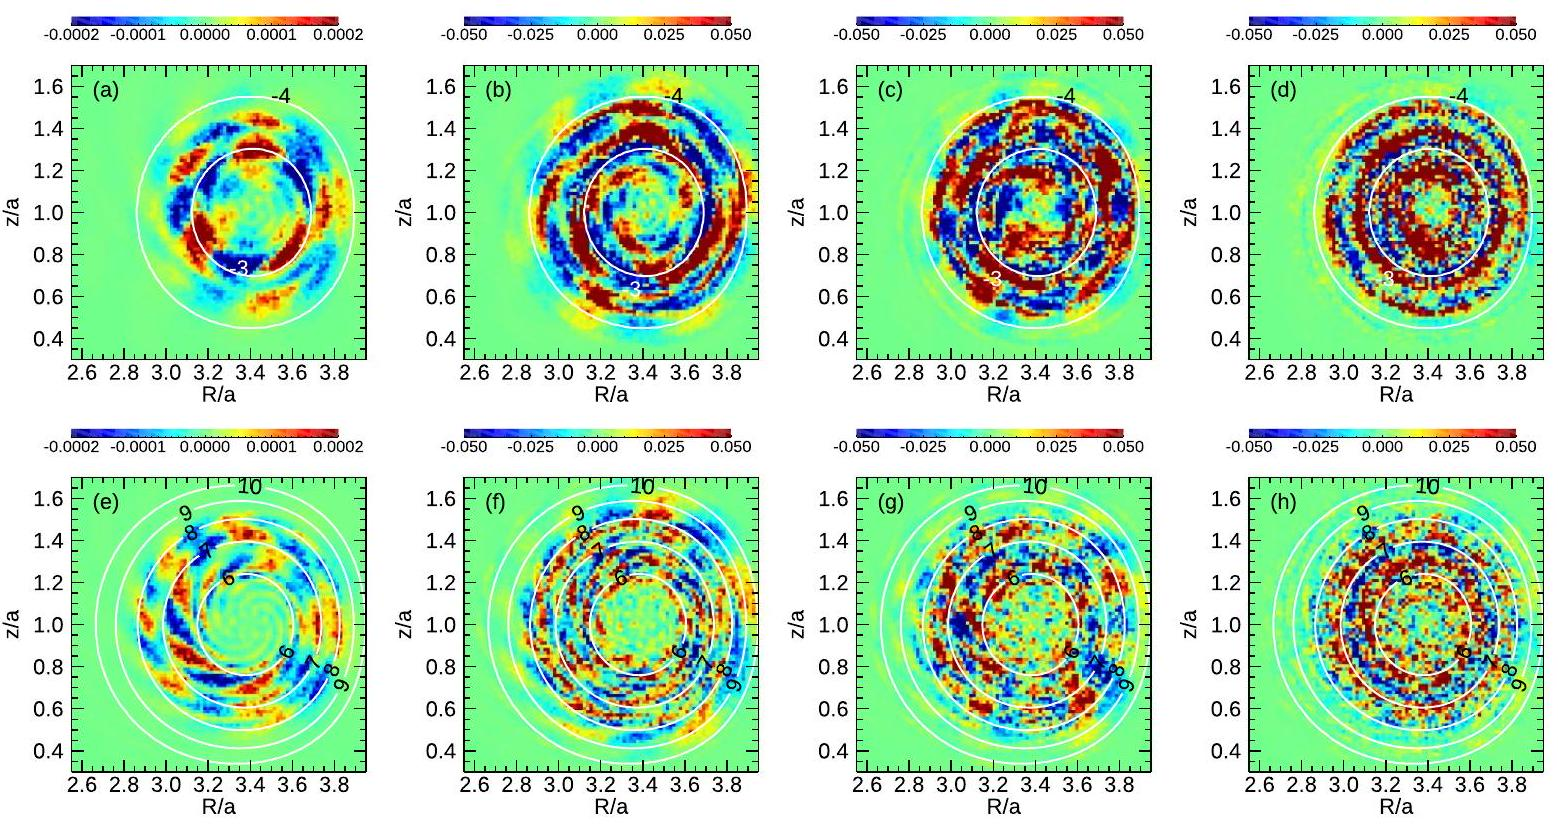
\includegraphics[max width=\textwidth, center]{2023_06_04_de2f4b8aa3fd859f006dg-13}

Figure 13. Thermal ion distribution function fluctuations in a poloidal plane $\left(R_{0}-0.65 a \leqslant R \leqslant R_{0}+0.75 a, z_{0}-0.7 a \leqslant z \leqslant\right.$ $\left.z_{0}+0.7 a, \varphi=0\right)$ with $R_{0}=3.2 a$ and $z_{0}=a$ for (a) (e) $\omega_{A} t=287$, (b, f) $\omega_{A} t=700$, (c, g) $\omega_{A} t=811,(\mathrm{~d}, \mathrm{~h}) \omega_{A} t=1150$ in the run for $\beta_{\text {bulk } 0}=4 \%$. Particle kinetic energy is $E=3.0 \times 10^{-2} m_{h} v_{A}^{2}$ and magnetic moment $\mu=0$. The top (bottom) panels show co-going (counter-going) particles to the plasma current. Resonant particle orbits are projected on the poloidal plane with the poloidal resonance number $L$ labeled in the figure for the $n=4$ TAE.

the resonance is not a dominant factor for the distribution function fluctuations of thermal ions. We can attribute this difference to the difference in poloidal resonance number. The poloidal resonance numbers labeled in figures 13 (a) and (e) are $L=-4,-3,6,7,8,9,10$ whose absolute values are close to the poloidal mode numbers of the $n=4$ TAE shown in figure 7(b). On the other hand, the poloidal resonance numbers labeled in figures 6(a) and (e) are $L=-2,-1,8,9,10,11,12$ whose absolute values are relatively far from the poloidal mode numbers of the $n=4$ TAE. These result in the difference in the strength of the interaction between thermal ions and the TAE. The thermal ion distribution function fluctuations shown in figures $13(\mathrm{~d})$ and (h) may be partially related to the resonance with the TAEs, but the structure is not so clear as those for energetic ions shown in figures $11(\mathrm{~d})$ and (h).

\section{Discussion and summary}
In this paper, we presented a new kinetic-MHD hybrid simulation model where the gyrokinetic PIC simulation is applied to both thermal ions and energetic particles. TAEs destabilized by energetic ions in tokamak plasmas are simulated with the new simulation model. We have demonstrated the energy channeling from energetic ions to thermal ions through AEs with the simulation. We analyzed the distribution function fluctuations and the resonance condition for both thermal ions and energetic ions. For energetic ions, the distribution function is flattened on the $E^{\prime}=$ const. line in the phase space location where the resonance condition is satisfied and the $\mathrm{AE}$ has a substantial amplitude. Here, $E^{\prime}$ is a conserved variable for the wave-particle interaction. The absolute value of the poloidal resonance number $|L|$ is close to the poloidal mode number of the AE $m$. This results in the strong energy transfer and the strong particle transport. Since the poloidal orbit frequency is positive in our definition $\left(\omega_{\vartheta}>0\right)$, the sign of $L$ and $m$ may be different from each other, and we assumed $m \geq 0$ in this work. On the other hand, when the bulk plasma beta is $1 \%$, the variations of thermal ion distribution function does not follow the resonance curves but appear along the $q=$ const. curves or on the magnetic surfaces. This indicates that thermal ions have the fluid-like response to the $\mathrm{AE}$ and the resonance does not play an important role. The fluid-like response can be attributed to the absolute value of the poloidal resonance number $|L|$ which is far from the poloidal mode number of the AE. For bulk plasma beta $4 \%,|L|$ for thermal ions is closer to the poloidal mode number of the TAE, and the resonance become important leading to Landau damping.

These results lead to the conclusion that the strong energy transfer between the particles and the $\mathrm{AE}$ and the strong particle transport occur when the following conditions are satisfied at the resonance location in phase space: (1) the absolute value of the poloidal resonance number $|L|$ is close to the poloidal mode number of the $\mathrm{AE}$, (2) the $\mathrm{AE}$ has a substantial amplitude, (3) the distribution function has a substantial gradient along the $E^{\prime}=$ const. line. In a uniform slab plasma, the net energy transfer arises only when the resonance condition is satisfied with $|L|=m$. In toroidal plasmas, however, the net energy transfer arises even for $|L| \neq m$, because the distribution function fluctuations with the poloidal mode number $L$ and the $\mathrm{AE}$ harmonics with poloidal mode number $m$ can couple in the volume integration for the energy transfer through the magnetic gradient and curvature drifts and the Jacobian of phase space, which contain poloidal mode numbers not equal to 0 . If $|L|$ is far from $m$, however, their coupling is weak and the resonance is not important for the distribution function fluctuations.

For the TAE investigated in this paper, we can conclude that the kinetic thermal ions are essential for $\beta_{\text {bulk } 0}=4 \%$, but are not for $\beta_{\text {bulk } 0}=1 \%$. With the new kinetic-MHD hybrid simulation presented in this paper, energy channeling from energetic particles to thermal ions through the EGAM [46, 47] and the stabilization of pressure driven instabilities in the Large Helical Device (LHD) plasmas by the kinetic effects of thermal ions [44, 45] have been demonstrated. The energeticparticle distribution function analyses in the simulations of AE bursts and frequency chirping have proved to be useful methods for elucidating the nonlinear physical mechanisms [55-57]. The distribution function fluctuation analysis presented in this paper is a powerful tool to elucidate the waveparticle interaction in toroidal plasmas. As we stated in the introduction section, MHD requires the kinetic extension for the application to the collisionless high-temperature plasmas. In a conventional hybrid simulation without kinetic thermal ions for $\beta_{\mathrm{bulk} 0}=4 \%$, which is not presented in this paper, we found that a pressure driven MHD mode is unstable and affects the TAE. This makes the comparison difficult between the conventional hybrid simulation and the new kinetic-MHD hybrid simulation for $\beta_{\text {bulk } 0}=4 \%$. This suggests an important stabilizing effect of kinetic thermal ions, which may be similar to that observed for LHD, but the analysis of the stabilizing mechanism is beyond the scope of this paper and transferred to our future work.

Though collisions are neglected in this work, collisions can be implemented for ion particle dynamics with the $\delta f$ simulation extended for collisions $[58,59]$. We should consider the consistency between collisions and dissipations such as viscosity and resistivity. For resistivity, a frictional force should be considered for ion dynamics to be consistent with the resistivity which arises from collisions between ions and electrons. In $[44,60]$, the ideal electric field without the resistive term was used for ion dynamics because the resistive part of the electric field is cancelled out with the frictional force. The total electric field with the resistive term was used for the induction equation which describes the magnetic field evolution. In this work, we used the total electric field with the resistive term for both the induction equation and the ion dynamics because the resistive component of the electric field is negligibly smaller than the ideal component for the AEs.

We introduced the parallel electric field in equation (11) given by the electron pressure gradient. This term is derived from the electron momentum equation neglecting the inertia term. We presented two models of electron pressure in this paper. One model assumes the time-independent electron temperature profile and the electron density whose charge density cancels out ion charge density. An additional electrostatic potential has been constructed, which gives the parallel and the perpendicular electric field, in terms of quasi-neutrality $[41,43]$. The parallel electric field adopted in this work is consistent with the quasi-neutrality model. In [43], the quasi-neutrality condition is extended with the ion polarization effect. The quasi-neutrality model also yields the perpendicular electric field of which $\mathbf{E} \times \mathbf{B}$ drift should be considered in the momentum vector given by equation (13). In addition, the electric field generated by the quasi-neutrality does not affect the magnetic field evolution since it is an electrostatic field. In [41], electrostatic modes and their coupling to the internal kink mode were studied. The quasi-neutrality condition will enable us to study electrostatic modes such as iontemperature-gradient (ITG) modes if the quasi-neutrality condition is appropriately implemented with the finite Larmor radius effects. A rich research field where the MHD modes and the electrostatic modes are coupled together will be open with the additional electrostatic potential. On the other hand, we adopted only the parallel electric field and neglected the perpendicular component in this work. This is a reasonable choice when we focus on the MHD modes without being disturbed with electrostatic modes. However, the code benchmark on electrostatic modes, for example, ITG modes with the implementation of the quasi-neutrality electric field is desired and will be conducted in the near future. We would like to emphasize that the new kinetic-MHD hybrid simulation will improve our understanding of many critical issues of tokamak and stellarator/heliotron plasmas and contribute to the prediction of burning plasmas.

\section{Data availability statement}
The data that support the findings of this study are available upon reasonable request from the authors.

\section{Acknowledgments}
We would like to thank Dr D A Spong, Dr L E Sugiyama, Dr Xian-Qu Wang, and Dr Jialei Wang for helpful discussions. Numerical computations were performed on the Plasma Simulator (FUJITSU FX100 and NEC SX-Aurora TSUBASA) of NIFS with the support and under the auspices of the NIFS Collaboration Research program (NIFS18KNST125, NIFS19KNXN396, NIFS20KNST169), the JFRS-1 of the International Fusion Energy Research Centre, and the K Computer and the Supercomputer Fugaku of the RIKEN Center for Computational Science (Project IDs: hp190190, hp200127, $\mathrm{hp}$ 210178). This work was supported by MEXT as Priority Issue on Post-K computer (Accelerated Development of Innovative Clean Energy Systems) and Program for Promoting Researches on the Supercomputer Fugaku (Exploration of burning plasma confinement physics).

\section{ORCID iDs}
Y Todo (iD) \href{https://orcid.org/0000-0001-9323-8285}{https://orcid.org/0000-0001-9323-8285}

M Sato (iD) \href{https://orcid.org/0000-0002-8921-961X}{https://orcid.org/0000-0002-8921-961X}

Hao Wang (iD) \href{https://orcid.org/0000-0002-9819-7483}{https://orcid.org/0000-0002-9819-7483}

R Seki (iD \href{https://orcid.org/0000-0002-5364-805X}{https://orcid.org/0000-0002-5364-805X}

\section{References}
[1] Park W et al 1992 Three-dimensional hybrid gyrokinetic-magnetohydrodynamics simulation Phys. Fluids B 4 2033-7

[2] Park W, Belova E V, Fu G Y, Tang X Z, Strauss H R and Sugiyama L E 1999 Plasma simulation studies using multilevel physics models Phys. Plasmas 6 1796-803

[3] Spong D A, Carreras B A and Hedrick C L 1992 Linearized gyrofluid model of the alpha-destabilized toroidal Alfvén eigenmode with continuum damping effects Phys. Fluids B $43316-28$

[4] Todo Y, Sato T, Watanabe K, Watanabe T H and Horiuchi R 1995 Magnetohydrodynamic vlasov simulation of the toroidal Alfvén eigenmode Phys. Plasmas 2 2711-6

[5] Briguglio S, Vlad G, Zonca F and Kar C 1995 Hybrid magnetohydrodynamic-gyrokinetic simulation of toroidal Alfvén modes Phys. Plasmas 2 3711-23

[6] Todo Y and Sato T 1998 Linear and nonlinear particle-magnetohydrodynamic simulations of the toroidal Alfvén eigenmode Phys. Plasmas 5 1321-7

[7] Fu G Y, Park W, Strauss H R, Breslau J, Chen J, Jardin S and Sugiyama L E 2006 Global hybrid simulations of energetic particle effects on the $n=1$ mode in tokamaks: internal kink and fishbone instability Phys. Plasmas $\mathbf{1 3} 052517$

[8] Kim C C 2008 Impact of velocity space distribution on hybrid kinetic-magnetohydrodynamic simulation of the $(1,1)$ mode Phys. Plasmas $\mathbf{1 5} 072507$

[9] Wang X, Zonca F and Chen L 2010 Theory and simulation of discrete kinetic beta induced Alfvén eigenmode in tokamak plasmas Plasma Phys. Control. Fusion 52115005

[10] Zhu J, Ma Z W and Wang S 2016 Hybrid simulations of Alfvén modes driven by energetic particles Phys. Plasmas 23122506

[11] Burby J W and Tronci C 2017 Variational approach to low-frequency kinetic-MHD in the current coupling scheme Plasma Phys. Control. Fusion 59045013

[12] Fu G Y and Park W 1995 Nonlinear hybrid simulation of the toroidicity-induced Alfvén eigenmode Phys. Rev. Lett. 74 1594-6

[13] Briguglio S, Schneller M, Wang X, Di Troia C, Hayward-Schneider T, Fusco V, Vlad G and Fogaccia G 2017 Saturation of Alfvén modes in tokamak plasmas investigated by Hamiltonian mapping techniques $\mathrm{Nucl}$. Fusion 57072001

[14] Briguglio S, Vlad G, Zonca F and Fogaccia G 2002 Nonlinear saturation of shear Alfvén modes and self-consistent energetic ion transport in burning plasmas with advanced tokamak equilibria Phys. Lett. A $\mathbf{3 0 2} 308-12$

[15] Todo Y 2006 Properties of energetic-particle continuum modes destabilized by energetic ions with beam-like velocity distributions Phys. Plasmas $\mathbf{1 3} 082503$

[16] Todo Y, Shinohara K, Takechi M and Ishikawa M 2003 Computer simulation of frequency sweeping of energetic particle mode in a JT-60u experiment J. Plasma Fusion Res. 791107

[17] Bierwage A, Shinohara K, Todo Y, Aiba N, Ishikawa M, Matsunaga G, Takechi M and Yagi M 2017 Self-consistent long-time simulation of chirping and beating energetic particle modes in JT-60u plasmas Nucl. Fusion 57016036

[18] Shiozaki Y and Todo Y 2004 Computer simulation of fishbone oscillation J. Plasma Fusion Res. Ser. 6 618-21 (available at: \href{http://www.jspf.or.jp/JPFRS/PDF/Vol6/jpfrs2004_06618.pdf}{http://www.jspf.or.jp/JPFRS/PDF/Vol6/jpfrs2004\_06618.pdf})

[19] Vlad G, Briguglio S, Fogaccia G, Zonca F, Fusco V and Wang X 2013 Electron fishbone simulations in tokamak equilibria using XHMGC Nucl. Fusion 53083008 [20] Pei Y, Xiang N, Youjun H, Y Todo G Li, Shen W and Liqing X 2017 Kinetic-MHD hybrid simulation of fishbone modes excited by fast ions on the experimental advanced superconducting tokamak (EAST) Phys. Plasmas 24032507

[21] Shen W, Feng Wang G Y Fu L X, Guoqiang Li and Liu C 2017 Hybrid simulation of fishbone instabilities in the EAST tokamak Nucl. Fusion 57116035

[22] Shen W, Feng Wang G Y Fu L X and Ren Z 2020 Hybrid simulation of fishbone instabilities with reversed safety factor profile $\mathrm{Nucl}$. Fusion $\mathbf{6 0} 106016$

[23] Brochard G, Dumont R, Lütjens H, Garbet X, Nicolas T and Maget P 2020 Nonlinear dynamics of the fishbone-induced alpha transport on ITER Nucl. Fusion 60126019

[24] Fu G Y 2008 Energetic-particle-induced geodesic acoustic mode Phys. Rev. Lett. 101185002

[25] Wang H and Todo Y 2013 Linear properties of energetic particle driven geodesic acoustic mode Phys. Plasmas 20012506

[26] Wang H, Todo Y and Kim C C 2013 Hole-clump pair creation in the evolution of energetic-particle-driven geodesic acoustic modes Phys. Rev. Lett. 110155006

[27] Wang H, Todo Y, Ido T and Osakabe M 2015 Simulation study of high-frequency energetic particle driven geodesic acoustic mode Phys. Plasmas 22092507

[28] Wang H, Todo Y, Ido T and Suzuki Y 2018 Chirping and sudden excitation of energetic-particle-driven geodesic acoustic modes in a large helical device experiment Phys. Rev. Lett. 120175001

[29] Todo Y, Van Zeeland M A, Bierwage A and Heidbrink W W 2014 Multi-phase simulation of fast ion profile flattening due to Alfvén eigenmodes in a diii-d experiment Nucl. Fusion 54104012

[30] Todo Y, Van Zeeland M A, Bierwage A, Heidbrink W W and Austin M E 2015 Validation of comprehensive magnetohydrodynamic hybrid simulations for Alfvń eigenmode induced energetic particle transport in diii-d plasmas Nucl. Fusion 55073020

[31] Todo Y, Van Zeeland M A and Heidbrink W W 2016 Fast ion profile stiffness due to the resonance overlap of multiple Alfvén eigenmodes Nucl. Fusion 56112008

[32] Bierwage A, Shinohara K, Todo Y, Aiba N, Ishikawa M Matsunaga G, Takechi M and Yagi M 2018 Simulations tackle abrupt massive migrations of energetic beam ions in a tokamak plasma Nat. Commun. 93282

[33] Todo Y, Seki R, Spong D A, Wang H, Suzuki Y, Yamamoto S, Nakajima N and Osakabe M 2017 Comprehensive magnetohydrodynamic hybrid simulations of fast ion driven instabilities in a large helical device experiment Phys. Plasmas 24081203

[34] Seki R, Todo Y, Suzuki Y, Spong D A, Ogawa K, Isobe M and Osakabe M 2019 Comprehensive magnetohydrodynamic hybrid simulations of Alfvén eigenmode bursts and fast-ion losses in the large helical device Nucl. Fusion 59096018

[35] Gorelenkov N N, Cheng C Z and Fu G Y 1999 Fast particle finite orbit width and larmor radius effects on low-n toroidicity induced Alfvén eigenmode excitation Phys. Plasmas 6 2802-7

[36] Lauber P, Günter S and Pinches S D 2005 Kinetic properties of shear Alfvén eigenmodes in tokamak plasmas Phys. Plasmas 12122501

[37] Zhang H S, Lin Z, Holod I, Wang X, Xiao Y and Zhang W L 2010 Gyrokinetic particle simulation of beta-induced Alfvén eigenmode Phys. Plasmas 17112505

[38] Chen Y, Munsat T, Parker S E, Heidbrink W W, Van Zeeland M A, Tobias B J and Domier C W 2013 Gyrokinetic simulations of reverse shear Alfvén eigenmodes in diii-d plasmas Phys. Plasmas 20012109 [39] Mishchenko A, Bottino A, Hatzky R, Sonnendrücker E, Kleiber R and Axel K 2017 Mitigation of the cancellation problem in the gyrokinetic particle-in-cell simulations of global electromagnetic modes Phys. Plasmas 24081206

[40] Biancalani A, Bottino A, Lauber P, Mishchenko A and Vannini F 2020 Effect of the electron redistribution on the nonlinear saturation of Alfvén eigenmodes and the excitation of zonal flows J. Plasma Phys. 86825860301

[41] Antonsen T M and Bondeson A 1993 Influence of trapped thermal particles on internal kink modes in high temperature tokamaks Phys. Fluids B 5 4090-8

[42] Graves J P, Hastie R J and Hopcraft K I 2000 The effects of sheared toroidal plasma rotation on the internal kink mode in the banana regime Plasma Phys. Control. Fusion 42 1049-66

[43] Lanthaler S, Graves J P, Pfefferlé D and Cooper W A 2019 Guiding-centre theory for kinetic-magnetohydrodynamic modes in strongly flowing plasmas Plasma Phys. Control. Fusion 61074006

[44] Sato M and Todo Y 2019 Effect of precession drift motion of trapped thermal ions on ballooning modes in helical plasmas Nucl. Fusion $\mathbf{5 9} 094003$

[45] Sato M and Todo Y 2020 Ion kinetic effects on linear pressure driven magnetohydrodynamic instabilities in helical plasmas J. Plasma Phys. 86815860305

[46] Wang H, Todo Y, Osakabe M, Ido T and Suzuki Y 2019 Simulation of energetic particle driven geodesic acoustic modes and the energy channeling in the large helical device plasmas Nucl. Fusion 59096041

[47] Wang H, Todo Y, Osakabe M, Ido T and Suzuki Y 2020 The systematic investigation of energetic-particle-driven geodesic acoustic mode channeling using MEGA code Nucl. Fusion 60112007

[48] Todo Y, Wang H and Sato M 2017 A new magnetohydrodynamic hybrid simulation model with thermal and energetic ions 26th Int. Toki Conf. (Toki, Japan, 5-8 December 2017) [49] Hazeltine R D and Meiss J D 1992 Plasma Confinement (Reading, MA: Addison-Wesley)

[50] Dimits A M and Lee W W 1993 Partially linearized algorithms in gyrokinetic particle simulation J. Comput. Phys. $107309-23$

[51] Parker S E and Lee W W 1993 A fully nonlinear characteristic method for gyrokinetic simulation Phys. Fluids B 5 77-86

[52] Aydemir A Y 1994 A unified monte carlo interpretation of particle simulations and applications to non-neutral plasmas Phys. Plasmas 1 822-31

[53] Todo Y 2019 Introduction to the interaction between energetic particles and Alfven eigenmodes in toroidal plasmas Rev. Mod. Plasma Phys. 31

[54] Hsu C T and Sigmar D J 1992 Alpha-particle losses from toroidicity-induced Alfvén eigenmodes. Part I: phase-space topology of energetic particle orbits in tokamak plasma Phys. Fluids B 4 1492-505

[55] Todo Y 2019 Critical energetic particle distribution in phase space for the Alfvén eigenmode burst with global resonance overlap Nucl. Fusion 59096048

[56] White R B, Duarte V N, Gorelenkov N N, Fredrickson E D and Podesta M 2020 Phase-space dynamics of Alfvén mode chirping Phys. Plasmas 27052108

[57] Wang X Q et al 2020 Nonlinear simulations of energetic particle-driven instabilities interacting with Alfvén continuum during frequency chirping Plasma Phys. Control. Fusion $\mathbf{6 3} 015004$

[58] Lin Z, Tang W M and Lee W W 1995 Gyrokinetic particle simulation of neoclassical transport Phys. Plasmas $22975-88$

[59] Wang W X, Nakajima N, Okamoto M and Murakami S 1999 A new bdeltafmethod for neoclassical transport studies Plasma Phys. Control. Fusion 41 1091-108

[60] Belova E V, Jardin S C, Ji H, Yamada M and Kulsrud R 2000 Numerical study of tilt stability of prolate field-reversed configurations Phys. Plasmas 7 4996-5006


\end{document}